\documentclass{SZTUthesis}
\usepackage{makecell}
\usepackage{algorithm}
\usepackage{algorithmicx}
\usepackage{setspace}
\usepackage{makecell}
\setstretch{1.5}
\hypersetup{
colorlinks=true,
linkcolor=black
}

\newcommand\pkg[1]{\texttt{#1}\textsuperscript{\sffamily PKG}}
\newcommand\env[1]{\texttt{#1}\textsuperscript{\sffamily ENV}}
\newcommand\app[1]{\textsf{#1}}
\newcommand\oper[1]{\texttt{#1}}
\newcommand\cls[1]{\texttt{#1}\textsuperscript{\sffamily CLS}}
\newcommand\bib[1]{\texttt{#1}\textsuperscript{\sffamily BIB}}
\renewcommand\emph[1]{\textbf{#1}}
\newcommand\format[1]{\textsf{#1}}

%算法
%\begin{algorithm}[t]
%\caption{algorithm caption} %算法的名字
%\hspace*{0.02in} {\bf Input:} %算法的输入, \hspace*{0.02in}用来控制位置,同时利用 \\ 进行换行
%input parameters A, B, C\\
%\hspace*{0.02in} {\bf Output:} %算法的结果输出
%output result
%\begin{algorithmic}[1]
%\State some description % \State 后写一般语句
%\For{condition} % For 语句,需要和EndFor对应
%    \State ...
%    \If{condition} % If 语句,需要和EndIf对应
%        \State ...
%    \Else
%        \State ...
%    \EndIf
%\EndFor
%\While{condition} % While语句,需要和EndWhile对应
%    \State ...
%\EndWhile
%\State \Return result
%\end{algorithmic}
%\end{algorithm}

%!TEX root = ../sztuthesis_main.tex
% 文章信息


% % 这里注意根据封面需要的样式手动用“\\”对标题断行
% 如果提示 “Overfull \\hbox (26.47823pt too wide)” 或和“题目:”不在同一行,
% 则说明有点宽,可调整断行
% \titlecn{测试短标题}
\titlecn{基于Springboot的弹幕视频网站后端系统\\设计与实现}
\titleen{Design and implementation of the back-end system of the barrage video website based on Springboot University}

\priormajor{物联网工程}
\author{潘俊霖}
\supervisor{孙瑞泽}
\supervisortitle{助理教授}
\department{大数据与互联网学院}
\studentid{202100201068}
\thesisdate{year=2025,month=5,day=5}



\clcnumber{TP391} 				% 中图分类号 Chinese Library Classification
\schoolcode{14655}			% 学校代码
\udc{004.9}						% UDC
\academiccategory{学术学位}	% 学术类别


\newif \ifblindreview % 条件语句,是否是盲审版本
% \blindreviewtrue
\blindreviewfalse

% lipsum
\newcommand{\lipsum}{%
这是一段随机插入的文本,用来填充模板布局,感受模板视觉效果。

深圳技术大学是广东省和深圳市高起点、高水平、高标准建设的本科层次公办普通高等学校。2015年,深圳市委市政府开始筹建深圳技术大学。2016年3月,深圳市人民政府办公厅发布关于设立深圳技术大学筹备办公室的通知。2017年7月,深圳市机构编制委员会发布关于设立深圳技术大学(筹)的通知。2017年9月、2018年9月深圳技术大学(筹)依托深圳大学分别招收了226人和807人。2018年11月30日,经教育部批准正式设立深圳技术大学,学校独立招生,标识码为4144014655,定位于应用型高等学校。2019年9月,学校首年独立招生录取807人,招生的六个省份均高于一本线(高优线/自招线)录取;其中,广东省理科投档线进入前十。

学校充分借鉴和引进德国、瑞士等发达国家一流技术大学先进的办学经验,致力于培养本科及以上层次具有国际视野、工匠精神和创新创业能力的高水平工程师、设计师等高素质应用型人才,努力建成一流的应用型技术大学。

着力建设面向国家和地方发展需要的,以工学为主,理学、管理学、艺术学等协调发展的学科体系,并按计划分布发展和优化学科布局。

目前设立了中德智能制造学院、大数据与互联网学院、新材料与新能源学院、城市交通与物流学院、健康与环境工程学院、创意设计学院、工程物理学院、质量和标准学院、国际交流学院、商学院、药学院、外国语学院、马克思主义学院(人文社科学院)、体育学院。已开设机械设计制造及其自动化、物联网工程、光源与照明、交通运输、汽车服务工程、工业设计等高度契合经济发展和产业需求的专业。至2022年,学校拟开设专业39个,涵盖工学、理学、管理学、艺术学、经济学等5个学科门类。

这是一段随机插入的文本,用来填充模板布局,感受模板视觉效果。%
}

% 让各类元素在全文按1、2、3...顺序编号,而不因章节变化而重置为1
\numberwithin{figure}{section}
\numberwithin{equation}{section}
\numberwithin{algorithm}{section}
\numberwithin{table}{section}

\begin{document}
%%%%%%%%%%%%%%%%%%%%%%%%%%%%%%%%%%%%%%%%%%%%%%%%%%
% 封面
% -----------------------------------------------%
\makecoverpage

%%%%%%%%%%%%%%%%%%%%%%%%%%%%%%%%%%%%%%%%%%%%%%%%%%
% 前置部分的页眉页脚设置
% -----------------------------------------------%
\newpage


\pagestyle{empty}
%%%%%%%%%%%%%%%%%%%%%%%%%%%%%%%%%%%%%%%%%%%%%%%%%%
% 声明页
% -----------------------------------------------%
\announcement
\newpage


% 目录
% -------------------------------------------%
{
\renewcommand{\contentsname}{\hfill \heiti \zihao{-2} 目\quad 录\hfill}  
    \zihao{4}
    \setlength{\parskip}{6pt}               % 段间距,补偿latex行间距计算(与word的差距)
    \renewcommand*{\baselinestretch}{1.5}   % 行间距
    \tableofcontents
}
\newpage

% 去掉页眉章节序号后面的“.”
\renewcommand{\sectionmark}[1]{\markright{\thesection~ #1}} 
\renewcommand{\headrulewidth}{1pt}



% 正文内容 
% --------------------------------------------%

\setheader

% 可以使用include命令导入tex文件,从而避免过多修改本文件。

% 论文正文是主体,主体部分应从另页右页开始,每一章应另起页。一般由序号标题、文字叙述、图、表格和公式等五个部分构成。

% 重新设置正文行间距,因为前置部分设置时候行间距被改过
\renewcommand*{\baselinestretch}{1.5}   % 几倍行间距
\setlength{\baselineskip}{16pt}         % 基准行间距

% 摘要
{
    \linespread{1.5}
    %%%%%%%%%%%%%%%%%%%%%%%%%%%%%%%%%%%%%%%%%%%%%%%%%%
    % 中文摘要
    \setabstractfooter

    %!TEX root = ../sztuthesis_main.tex
% 设置中文摘要

\phantomsection
\addcontentsline{toc}{section}{摘要}

\keywordscn{Springboot;视频在线播放;弹幕系统}
\categorycn{TP391}
\begin{abstractcn}
    随着网络技术的发展,视频成为信息传播与娱乐消费的核心载体,用户对视频平台的互动性需求日益增长。本文基于 Springboot框架设计并实现了弹幕视频网站后端系统。该系统以视频在线播放为基础,弹幕功能为核心,综合运用 MySQL、FastDFS、WebSocket、Elasticsearch等技术,为用户提供视频播放、弹幕交互、点赞收藏等功能,满足用户多样化需求。系统采用微服务架构,具备良好的性能、可用性、安全性、可拓展性和可维护性。
\end{abstractcn}
    \newpage

    %%%%%%%%%%%%%%%%%%%%%%%%%%%%%%%%%%%%%%%%%%%%%%%%%%
    % 英文摘要
    % -----------------------------------------------%
    %!TEX root = ../sztuthesis_main.tex
\phantomsection
\addcontentsline{toc}{section}{Abstract}

\keywordsen{SpringBoot;Video online play;Barrage system}
\categoryen{TP391}
\begin{abstracten}
    With the development of network technology, video has become the core carrier of information dissemination and entertainment consumption, and users' demand for interactivity on video platforms is growing. This paper designs and implements the back-end system of the barrage video website based on the Springboot framework. The system is based on online video playback and the barrage function as the core. It uses MySQL, FastDFS, WebSocket, Elasticsearch and other technologies to provide users with functions such as video playback, barrage interaction, likes and collections to meet the diverse needs of users. The system adopts a microservice architecture with good performance, availability, security, scalability and maintainability.
\end{abstracten}
}
\setfooter
% 正文
{
% 表格字号应比正文小,这里设为五号,但是暂时没法在cls里设置(不然会影响到封面等tabular环境)
% 所以目前只好在主文件里局部\AtBeginEnvironment
    \AtBeginEnvironment{tabular}{\zihao{5}}
    
    \linespread{1.5}

    % 正文内容
     
    \begin{spacing}{1.5}
        %!TEX root = ../sztuthesis_main.tex
% 论文正文是主体,主体部分应从另页右页开始,每一章应另起页。一般由序号标题、文字叙述、图、表格和公式等五个部分构成。
\section{引言}

\subsection{研究背景与意义}

随着5G、云计算与边缘计算等新一代网络技术的高速发展与推广,当今的互联网内容生态正经历从图文静态展示向动态视频交互的变革。视频媒介凭借视听一体化的沉浸式体验,大幅降低了用户信息处理成本,契合当下碎片化时代的认知习惯,已成为信息传播与娱乐消费的核心载体。据第55次《中国互联网络发展状况统计报告》\cite{RN01}显示,截至2024年12月,我国网民规模达11.08亿人,在文旅娱乐类应用的分类中,网络视频用户规模达10.70亿人,占网民整体的96.6\%,远高于同分类下的其他应用,充分印证了当前互联网内容生态以视频媒介为主导的现状。

在Web3.0与元宇宙技术浪潮推动下,互联网正从信息交互的1.0时代向价值交互的3.0时代跃迁,用户对视频平台的需求也随之发生深刻变革。相较于早期以内容单向输出为主的视频网站,如今的用户更倾向于在观看过程中获得深度参与感与沉浸式社交体验\label{用户交流}。这种需求的转变,不仅体现在对高清画质、流畅播放等基础功能的追求上,更聚焦于构建双向互动、实时共享的虚拟空间。

弹幕作为实时互动的典型创新,通过即时评论叠加形成群体共鸣,打破了传统视频观看的时空壁垒。在观看视频时,用户发送的弹幕会以动态文字的形式实时叠加在视频画面上,让不同地域、不同时间的观众得以在同一虚拟空间中交流互动。这种 “边看边聊” 的模式,将原本孤立的观看行为转化为集体参与的社交活动,创造出独特的虚拟社交场域。用户不再是被动的内容接收者,而是成为内容传播与共创的重要参与者。

这种实时交互模式不仅显著提升了用户参与感,更催生出丰富的衍生文化现象。例如,热门视频中的经典台词、精彩片段往往会通过弹幕传播形成网络热梗,进而引发二次创作热潮。用户基于弹幕内容进行的二次创作,如剪辑、配音、图文解析等,进一步扩大了视频内容的传播范围与影响力。此外,弹幕文化还形成了独特的语言体系与互动规则,如 “前方高能”“弹幕护体” 等特定用语,成为Z世代网络社交的重要符号。弹幕不仅是一种互动方式,更成为Z世代表达自我、寻找同好、构建社群的重要载体,深刻影响着当代网络文化的发展走向。因此在用户需求持续迭代与行业竞争加剧的背景下,视频平台不仅需要保障视频播放流畅,画质清晰等的基础功能,平台还需要拓展以弹幕功能为核心的实时评论、用户互动、社交分享等功能。

随着5G、云计算技术的普及,互联网视频内容生产呈现多元化格局。其中职业生产内容(Occupationally Generated Content OGC)依托专业团队输出精品版权作品,用户生产内容(Professionally Generated Content,UGC)借助移动设备记录生活百态,专业生产内容(Professionally Generated Content,PGC)则由 MCN 机构打造兼具专业性与娱乐性的优质内容。\cite{1023409711.nh}多元生产模式推动视频内容爆发式增长,主流平台日均新增视频量突破千万级。面对海量内容,传统分类浏览已无法满足用户需求\label{互联网内容爆炸}。在此背景下,检索系统成为了视频平台必不可缺的一部分功能。

基于以上分析,本文设计并实现了一个基于Springboot的视频弹幕网站,它不仅能实现视频在线播放的基础功能,同时还添加了视频弹幕推送、投币、评论等的互动功能。


\subsection{国内外研究现状}

当前,全球多数视频网站的核心业务聚焦于视频内容供应,通过会员付费、广告投放等模式,为用户提供视听服务。在这一竞争格局下,优质内容已然成为行业竞争的关键要素。各平台主要通过自制或引进热门视频资源吸引用户,但在视频功能拓展方面投入相对不足,如用户观点交互渠道搭建、视频创作参与度提升等领域的开发仍有待加强。

从用户粘性角度来看,缺乏互动的单向视频观看模式,使得平台过度依赖内容数量与质量维系用户留存。视频内容的生产与版权采购成本高昂,自制内容面临同质化、制作经验匮乏、意识形态把控不足等挑战;版权采购则加剧平台间的竞争,进一步推高运营成本。

在国际视频平台中,YouTube 以专业用户生产内容(PUGC)为特色,内容多元且国际化程度高。平台通过创作者激励机制,营造浓厚的原创氛围,相较于传统内容采购模式,有效降低版权成本。但该平台功能相对单一,缺乏弹幕互动、博客发布等社交功能,用户与订阅者的互动基本局限于视频投稿。\cite{RN03}Netflix 作为全球最大的付费视频平台,凭借早期 DVD 租赁业务积累的用户付费习惯,成功实现向线上平台的转型。平台始终将优质内容视为发展核心,以会员订阅为主要营收来源,凭借高质量的剧集内容,吸引大量付费用户。然而,对内容品质的过度依赖,使得版权采购成本居高不下,且需持续产出优质内容以维持用户粘性。

国内视频平台如哔哩哔哩,初期聚焦二次元内容创作与分享,近年来通过拓展内容分区实现多元化发展,平台内容形成了以UGC和PGC为核心,PGC为辅的局面。依托兴趣社区的运营优势,哔哩哔哩在弹幕互动、用户社交等方面表现突出,高互动率形成正向循环,持续吸引用户参与。但受发展历程影响,其内容覆盖领域相对较窄,主要集中于年轻用户偏好的领域,难以满足全年龄段用户的观看需求。反观国内其他主流视频网站如爱奇艺、腾讯视频等,多采用专业生产内容(PGC)模式,与Netflix的运营逻辑相似,版权竞争激烈。与此同时,普遍存在内容质量欠佳、社区运营薄弱等问题,叠加高成本内容投入、单一盈利模式等因素,导致行业整体长期处于亏损状态,会员付费与广告收入难以覆盖内容制作与版权采购成本。

\subsection{主要研究内容}

\begin{enumerate}[label=(\arabic*)]
    \item 对国内外视频平台发展现状进行了分析,设计并实现了以视频在线播放为基础功能、弹幕功能为核心的视频弹幕网站后端系统,为用户提供了一个在线看视频同时还能进行弹幕交互的平台。
    \label{系统目标}
    \item 为用户提供了包括点赞、收藏、投币、关注等的一系列交互功能。同时还进一步添加了弹幕查询、在线人数查询、全局内容搜索、观看记录等功能。
    \end{enumerate}

\subsection{论文组织结构}

全文内容共四章,具体内容组织如下:

第一章为前言。介绍了本文的研究背景与意义,以及国内外相关研究现状,阐明了主要研究内容。

第二章为相关技术分析。介绍了本文实现视频弹幕网站所用涉及到的相关技术。

第三章为需求分析。对本文所实现的视频弹幕网站后端系统从功能性和非功能性两个角度进行需求分析。

第四章为系统设计。

第五章为系统实现。

第六章总结与展望,总结了本文的主要工作,展望了下一阶段的研究方向。

\newpage

\section{相关技术分析}
\subsection{SpringBoot}

SpirngBoot是基于Spring框架构建的开发框架,旨在简化Java应用的开发与配置,帮助使用者快速打造独立、生产级别的应用程序,在当今后端开发领域应用广泛。

它采用“约定优于配置”的原则,通过自动配置机制,能够自动装配数据库连接、Web服务器等组件,大幅减轻了开发者的配置负担\label{SpringBoot特性};提供丰富的启动器,可以快速搭建项目,让开发者能够专注业务逻辑;支持将应用打包成为可执行的JAR或WAR文件独立运行,简化了开发者的部署流程;同时还支持微服务架构,继承众多即插即用的功能,便于微服务的独立部署与拓展,显著提升了开发效率和应用的可用性。

\subsection{MySQL数据库}

MySQL数据库是一个开源的关系型数据库管理系统,它能够为开发者提供高效、可靠的数据存储和管理功能,现在属于Oracle公司。它以其中高性能、可靠性和易用性而闻名,被广泛应用于从个人网站到大型企业级应用的各种规模应用。

MySQL数据库主要具有高性能、可拓展性、安全性、易用性、跨平台、开源和社区支持等特点。\cite{RN04}
\begin{enumerate}[label=(\arabic*)]
    \item 高性能:MySQL被设计用于处理高并发和大数据量的应用,支持如nnoDB、MyISAM等多种储存引擎,能够提供快速的数据读写能力同时通过索引、查询优化和缓存机制,MySQL能够高效地处理复杂的查询和事务。
    \item 可拓展性:MySQL支持主从复制和分片技术,能够轻松拓展数据库的容量和性能,适合大型应用。通过增加更多服务器(水平拓展)和增加单个服务器的资源(垂直拓展),MySQL能够满足不断增长的数据请求。
    \item 安全性:MySQL提供多种安全特性,如用户权限管理,SSL加密、数据加密等,能够确保数据的安全性。同时通过细粒度的权限控制,MySQL能够保护敏感数据免于遭受未授权的访问。
    \item 易用性:依赖于命令行工具和MySQL Workbench这一类的图形化管理工具,使得数据库的管理和操作都变得简单。开发者可以轻松地创建、修改和查询数据库,但无需深入了解复杂的数据库知识。
    \item 跨平台:MySQL可以在包括Windows、Linux、macOS等多种操作系统上运行,提供良好的跨平台兼容性。这使得开发者能够在不同开发环境中使用MySQL而无需担心兼容性问题。
    \item 开源和社区支持:作为一款开源的数据库管理系统,MySQL拥有活跃的社区支持,开发者可以从中获取丰富的教程、文档和插件。同时社区驱动的开发模式也使得MySQL能够快速响应市场需求,从而不断地改进和更新。
\end{enumerate}

\subsection{FastDFS分布式存储}

FastDFS是一款基于C语言开发的轻量级开源高性能分布式文件系统。主要功能包含文件存储、文件同步、文件访问(上传/下载)。FastDFS解决了在大容量场景下的文件存储和高并发访问的问题,同时是了文件存储时的负载均衡,特别适合以文件为载体的中大型网站的在线服务,如照片共享网站、视频共享网站等(图片、文档、音频、视频等)。\cite{RN05}

和其他的分布式文件系统相比较,FastDFS文件系统通过取消了存储元数据的服务器,实现了元数据的可内存化,达到了提高检索效率的目的。如图\ref{The architecture of FastDFS}所示,FastDFS文件系统总共分为了跟踪服务器(Tracker Server)、存储服务器(Stroage Server)和客户端(client)三部分。\cite{RN06}
\begin{figure}[hbt]
    \centering
    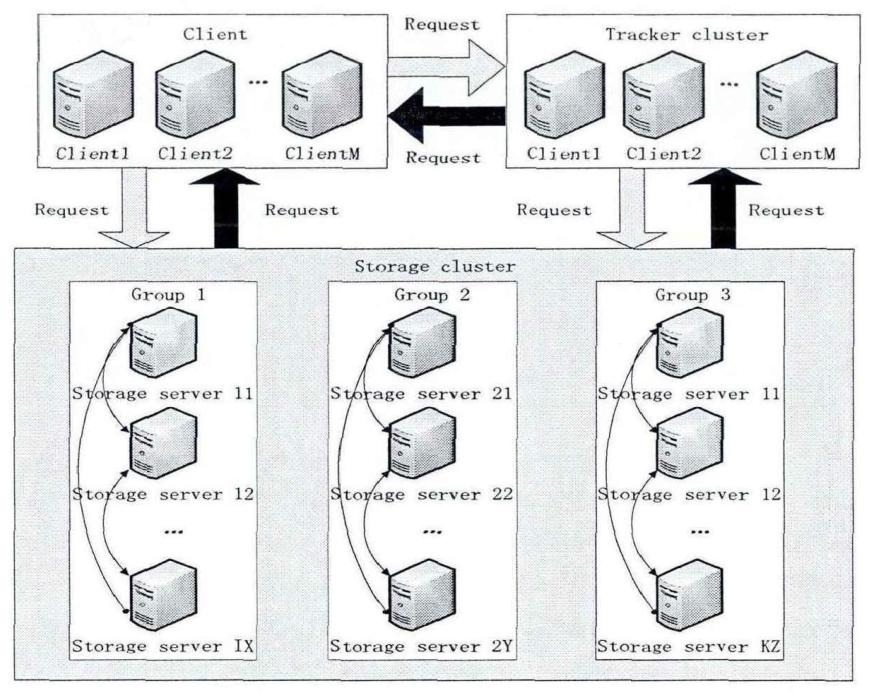
\includegraphics[width=0.5\textwidth]{The architecture of FastDFS.jpeg}
    \caption{FastDFS架构图}
    \label{The architecture of FastDFS}
    \end{figure}

FastDFS分布式存储主要有着高性能、高可用和易拓展的特点。
\begin{enumerate}[label=(\arabic*)]
    \item 高性能:从设计之初FastDFS就致力于处理高并发的文件上传和下载请求,通过文件分片和负载均衡技术,它能够高效地处理大小文件,支持大量的文件存储和访问,提供快速的文件读写能力。
    \item 高可用性:FastDFS采用了主从架构,支持文件冗余存储,这确保了在某个节点发生故障时文件仍然可用。并且FastDFS还通过心跳检测和自动故障转移这两个机制,保证了系统的稳定性和可靠性。
    \item 易拓展性:为满足不断增长的文件存储需求,FastDFS支持动态拓展存储节点,因此能轻松增加存储容量。开发者可以通过简单的配置就可以实现快速部署和拓展FastDFS集群。
\end{enumerate}

\subsection{WebSocket实时通信}

WebSockets是一种网络通讯协议,被用于在Web应用程序中实现实时、双向的通信通道。\cite{EN01}与传统的HTTP请求的一次请求一次响应不同,WebSocket允许服务器和客户端之间建立一个持久连接,允许服务器即时向客户端推送数据同时也就可以接收客户端发送的数据,实现实时数据传输。

如\ref{WebSocket principal}所示,WebSocket建立在普通的HTTP协议上,所有的WebSocket请求都会通过普通的HTTP协议发送出去,WebSokcet通过HTTP/1.1协议中的Upgrade头信息来告诉服务器,希望协议从HTTP/1.1升级到WebSocket协议\cite{RN07}。服务器会根据HTTP协议识别特定头信息Upgrade,同时也会判断请求信息中的Upgrade是否存在。在这个过程中HTTP协议是必不可少的。
\begin{figure}[hbt]
    \centering
    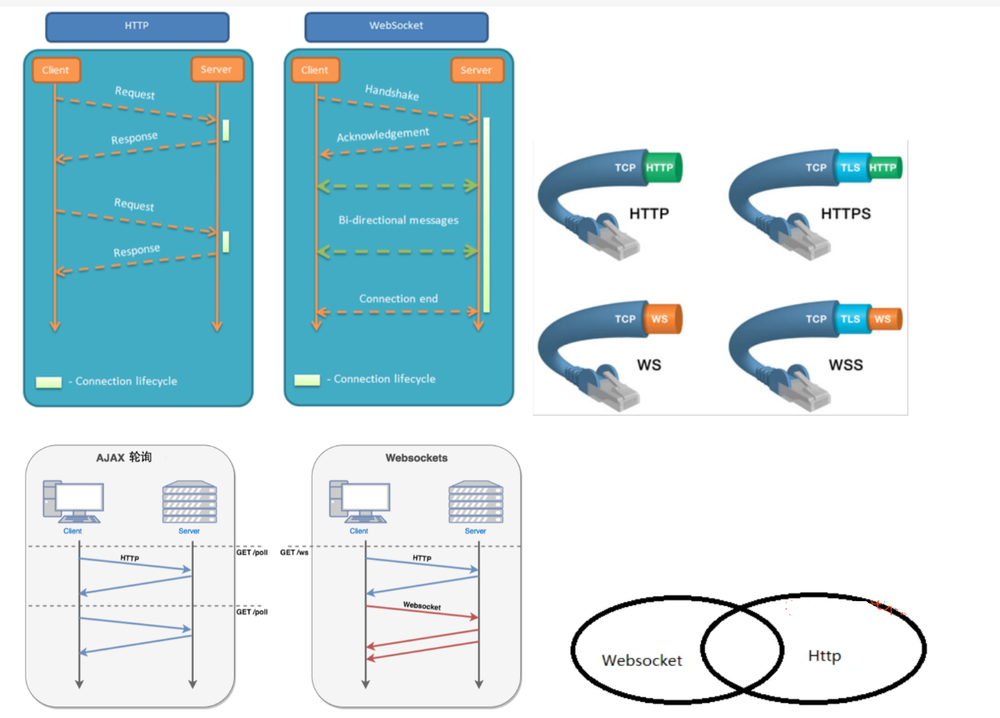
\includegraphics[width=0.5\textwidth]{WebSocket principal.png}
    \caption{WebSocket原理}
    \label{WebSocket principal}
    \end{figure}

开发者可以通过WebSocket的使用构建更加动态和响应迅速的Web应用,达到提升用户体验的目的。

\subsection{Elasticsearch搜索引擎}

Elasticsearch是一个基于Lurcene库构建的开源搜索引擎。提供了强大的全文搜索、结构化搜索、分析功能,被广泛应用于日志分析、实时监控、数据挖掘等领域。它通过RESTful接口提供搜索结果。Elasticsearch的分布式架构将索引细分为多个分片,这些分片随后可复制到集群内的多个服务器(节点)上。正因如此,Elasticsearch 能够应对高查询负载,平均分配处理负载,并弥补任何服务器故障带来的影响。这种架构支持即使在高负载情况下,搜索结果也能及时反映数据变化\cite{EN02}。

像亚马逊这样的大型企业提供专门的Elasticsearch服务,Github和StackOverflow都成功使用了这款搜索和分析引擎。通过Elasticsearch项目能够满足用户对快速、准确搜索的需求。
\newpage

\section{需求分析}

\subsection{业务概述}

在快节奏的现代生活中,视频凭借其生动形象的特点,逐渐成为人们获取信息、放松娱乐的首选方式。相较于单调的文字与静态的图片,视频融合了画面与声音,能为人们带来更加丰富和沉浸式的体验。人们可以借助视频学习各类知识,在忙碌的工作之余通过观看有趣的视频缓解压力,还能在探索不同视频内容的过程中培养新的兴趣爱好。

然而,随着网络技术的迅猛发展,网络上的视频数量呈现出爆炸式增长\ref{互联网内容爆炸}。面对数以亿计的视频资源,用户想要找到自己真正感兴趣的内容变得愈发困难。而且,不同用户查找视频的习惯大相径庭。部分用户偏好通过浏览自己感兴趣的视频分类来筛选内容;有些用户则更倾向于在搜索框中输入关键词进行查找;还有一些用户不喜欢主动搜索,期望视频网站能依据自身喜好,精准地为其推荐可能感兴趣的视频。由此可见,视频网站只有实现上述功能,才能满足不同用户的多样化需求。

此外,互联网的蓬勃发展不仅改变了人们获取信息的方式,还极大地激发了人们的社交欲望\ref{用户交流}。如今,人们在观看视频时,不再仅仅满足于被动观看,而是迫切希望表达自己对视频内容的独特见解,与其他用户进行互动交流。在这样的趋势下,视频网站若仅提供基础的视频观看功能,显然无法满足用户的需求。因此搭建多样化的视频评价渠道和社交平台,成为视频网站发展的必然趋势。这不仅有助于促进用户之间的思想交流,进一步提升网站视频的质量,还能增强用户对网站的认同感和归属感,有效提高视频网站的用户粘合度,使网站在竞争激烈的网络环境中占据优势地位。 

\subsection{功能性需求分析}

弹幕视频网站后端系统的目标非常明确,即通过建立弹幕视频网站平台,实现以视频在线播放为基础功能、弹幕功能为核心的视频弹幕网站后端系统,为用户提供了一个在线看视频同时还能进行弹幕交互的平台\ref{系统目标}。

根据系统目标,可以明确弹幕视频网站后端系统的功能性需求主要有五个,分别是用户管理、视频管理、社交功能、权限管理、搜索功能和实时通信功能模块。

\subsubsection{用户管理需求}

如\ref{用户管理用例图}所示,用户管理功能包括用户注册、用户登录、用户信息管理和用户角色管理这四个功能。
\begin{figure}[hbt]
    \centering
    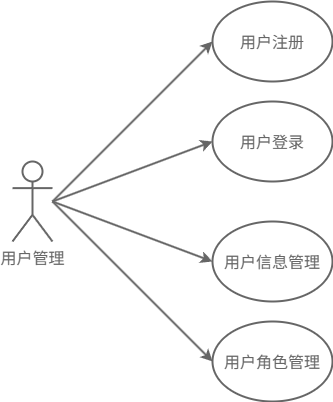
\includegraphics[width=0.5\textwidth]{用户管理.png}
    \caption{用户管理用例图}
    \label{用户管理用例图}
\end{figure}

用户注册功能旨在为用户创建在本系统内的专属账户,实现用户身份的唯一标识与管理,为用户使用系统各项功能提供前提条件。用户在注册页面输入用户名、密码、邮箱等必要信息,其中用户名需遵循系统规定的命名规范,密码需达到一定强度要求,邮箱必须为有效的邮箱地址。系统对用户输入的信息进行有效性验证,若全部有效,系统将创建新的用户账户,并将相关信息存储至数据库,同时向用户返回 “注册成功” 的提示信息;若信息存在无效情况,系统将返回相应的错误信息,提示用户重新输入正确信息。

用户登录功能是用户访问系统的入口,通过验证用户身份,确保只有授权用户能够使用系统的各项功能,保障系统的安全性和用户数据的保密性。用户在登录页面输入注册时使用的用户名和密码,系统将其与数据库中存储的信息进行匹配验证。若匹配成功,系统允许用户登录,并返回 “登录成功” 的信息,同时为用户生成会话标识,用户可凭借此标识在会话期间访问系统功能;若不匹配,系统返回错误提示,阻止非法访问。

用户信息管理功能允许已登录用户查看和修改个人信息,满足用户个性化需求,确保用户信息的准确性和时效性。用户登录系统后,通过导航菜单进入个人信息页面,可查看当前已有的个人信息。如需修改,可在相应编辑区域对用户名、密码、邮箱等信息进行修改,完成修改并提交后,系统保存修改后的信息,并返回 “更新成功” 的提示,确认信息修改操作已成功执行。

用户角色管理功能由系统管理员负责操作,通过对用户角色的管理和权限分配,实现系统资源的合理访问控制,确保系统的正常运行和数据安全。系统管理员登录系统后,进入用户角色管理页面,可查看当前系统中所有用户的角色列表。管理员根据业务需求,为用户分配新的角色或移除已有的角色,完成操作后,系统保存角色分配信息。

\subsubsection{视频管理需求}

如\ref{视频管理用例图}所示,视频管理功能包括视频上传、视频播放、弹幕功能这三个功能。
\begin{figure}[hbt]
    \centering
    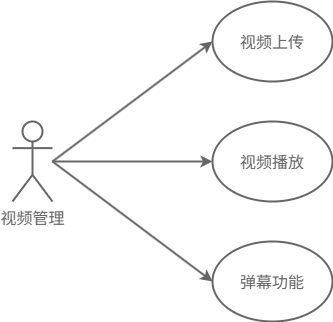
\includegraphics[width=0.5\textwidth]{视频管理.png}
    \caption{视频管理用例图}
    \label{视频管理用例图}
\end{figure}

视频上传功能赋予用户向系统提交视频文件的权限,丰富系统的视频资源库,满足用户分享内容的需求。用户登录系统后,通过导航菜单进入视频上传页面。在此页面,用户可选择本地要上传的视频文件。系统随即对所选视频文件的格式和大小进行严格验证,确保其符合系统预设的标准。若视频文件符合要求,系统会将其上传至存储系统,并向用户返回“上传成功”的提示信息;若不符合要求,系统会返回具体的错误信息,如“文件格式不支持,请选择正确格式的视频文件”或“文件大小超出限制,请选择合适大小的视频”,引导用户重新选择文件。 

视频播放功能为用户提供了观看已上传视频的服务,满足用户的视听娱乐需求。用户登录系统后,进入视频播放页面。在该页面,用户可从众多视频资源中选择想要播放的视频。系统接收到用户的选择指令后,会快速加载所选视频文件,并自动开始播放。播放过程中,用户可通过播放控制按钮,如播放、暂停、音量调节、进度拖动等,灵活控制视频播放,获得个性化的观看体验。 

弹幕功能增强了用户在视频观看过程中的互动体验,促进用户之间的交流与分享。当用户在视频播放页面观看视频时,可在专门的输入区域输入弹幕内容。输入完成后,用户点击发送按钮,系统会将弹幕信息发送到服务器。服务器借助WebSocket技术,将弹幕信息实时推送给所有正在观看该视频的用户。这些弹幕会在视频播放界面上以动态形式显示,用户不仅能看到自己发送的弹幕,还能实时浏览其他用户发送的弹幕,实现用户之间的实时互动交流。 

\subsubsection{社交功能需求}

如\ref{社交功能用例图}所示,社交功能包括用户关注、用户动态、用户硬币这三个功能。
\begin{figure}[hbt]
    \centering
    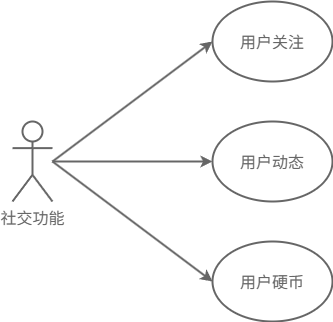
\includegraphics[width=0.5\textwidth]{社交功能.png}
    \caption{社交功能用例图}
    \label{社交功能用例图}
\end{figure}

用户关注功能为用户搭建起社交关系网络,方便用户与其他用户建立联系,拓展社交圈子。用户登录系统后,通过搜索或浏览等方式进入其他用户的个人主页。在对方的个人主页上,用户点击 “关注” 按钮,系统会迅速将这一关注请求发送到服务器。服务器接收到请求后,对其进行处理,更新该用户的关注列表,同时也会更新被关注用户的粉丝列表。完成处理后,系统返回 “关注成功” 的信息,此时用户在自己的关注列表页面,即可看到刚刚关注的用户,成功建立起与其他用户的关注关系。

用户动态功能给予用户分享自身状态、见解以及各类内容的平台,促进用户间的信息交流与互动。用户登录系统后,找到并进入动态发布页面。在这个页面中,用户可以在输入框内输入想要分享的动态内容,还能根据需求选择添加本地的图片或视频来丰富动态展示效果。当用户完成内容编辑后,点击 “发布” 按钮,系统会将包含文字、图片或视频等的动态信息发送到服务器。服务器接收到信息后,将其保存至数据库,并向用户返回 “发布成功” 的提示。随后,用户发布的动态不仅会展示在自己的个人主页上,还会出现在关注者的动态流中,让关注者能够及时看到该用户的分享内容,实现用户间的信息共享与互动。

用户硬币作为一种虚拟资产功能,为用户提供了购买内容或打赏其他用户的途径,激励内容创作与平台互动。用户登录系统后,通过导航栏找到并进入硬币管理页面。在此页面,用户能够直观地看到当前自己拥有的硬币数量。若用户有购买内容或打赏其他用户的需求,可在页面中选择相应的操作选项,并按照提示完成后续步骤。系统接收到用户的硬币使用请求后,会对请求进行处理,从用户的硬币余额中扣除相应数量,并同步更新用户的硬币余额数据,完成操作后返回 “使用成功” 的信息,告知用户硬币已成功使用。

\subsubsection{权限管理需求}

如\ref{权限管理用例图}所示,权限管理功能包括角色管理、菜单管理、操作权限管理这三个功能。
\begin{figure}[hbt]
    \centering
    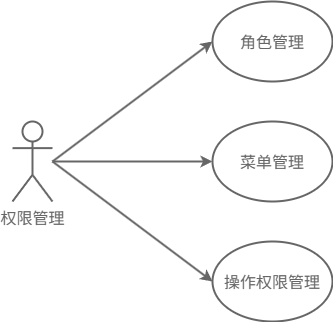
\includegraphics[width=0.5\textwidth]{权限管理.png}
    \caption{权限管理用例图}
    \label{权限管理用例图}
\end{figure}

角色管理功能赋予系统管理员对系统内角色进行全面管控的能力,通过创建、修改和删除角色,并合理分配权限,实现对不同用户群体访问系统资源和执行操作的精细控制,确保系统的安全性和稳定性。系统管理员登录系统后,通过特定的入口进入角色管理页面。在该页面,管理员能够查看当前系统中已存在的角色列表,了解各个角色的基本情况。若需要创建新角色,管理员可进行相应操作,设置角色名称和描述,明确该角色的功能和适用场景。对于现有角色,管理员可以根据实际业务需求,对角色名称、描述等信息进行修改。当某些角色不再适用于系统时,管理员可将其删除。在完成上述任何操作后,系统会保存角色信息,并向管理员返回 “更新成功” 的提示,确认角色管理操作已生效。

菜单管理功能让系统管理员能够灵活管理系统菜单,通过设置不同角色对菜单项的访问权限,实现系统界面展示的个性化和资源访问的安全性。系统管理员登录系统后,进入菜单管理页面。在此页面,管理员可以查看当前系统的菜单列表,清晰了解菜单的构成和布局。管理员可根据业务需求创建新菜单项,设置菜单名称、路径和图标,使新菜单项能够准确对应相应的功能模块,并在界面上有清晰的展示。对于已有的菜单项,若有调整需求,管理员可以修改其名称、路径等信息。对于不再使用的菜单项,管理员可将其删除。系统在保存这些菜单信息变更后,会返回 “更新成功” 的信息,告知管理员菜单管理操作已成功完成。

操作权限管理功能帮助系统管理员对系统内的操作权限进行有效管理,通过明确不同角色可执行的操作,保障系统的正常运行和数据安全。系统管理员登录系统后,进入操作权限管理页面。在该页面,管理员可以查看当前系统的操作权限列表,掌握各个操作权限的设置情况。当业务需要新的操作权限时,管理员可以创建新操作权限,详细设置权限名称和描述,界定该权限的具体作用。对于已有的操作权限,管理员可以根据实际情况修改其名称、描述等信息。若某些操作权限不再使用,管理员可将其删除。系统在保存操作权限信息的变动后,会返回 “更新成功” 的信息,表明操作权限管理操作已顺利执行。

\subsubsection{搜索功能需求}

如\ref{搜索功能用例图}所示,搜索功能包括视频搜索和数据分析这两个功能。
\begin{figure}[hbt]
    \centering
    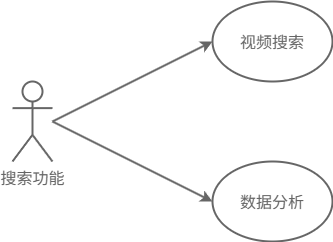
\includegraphics[width=0.5\textwidth]{搜索功能.png}
    \caption{搜索功能用例图}
    \label{搜索功能用例图}
\end{figure}

视频搜索功能为用户提供了在海量视频资源中快速定位所需内容的途径,满足用户对特定视频的查找需求。用户登录系统后,通过导航栏或快捷入口进入搜索页面。在搜索页面的搜索框中,用户输入想要查找视频的关键词,这些关键词可以是视频标题中的字词、视频描述里的关键信息等。输入完成后,用户点击 “搜索” 按钮,系统会将包含关键词的搜索请求发送到服务器。服务器借助Elasticsearch强大的全文搜索能力,在视频数据库中进行精准查找,筛选出与关键词相关的视频。随后,系统将搜索到的视频结果展示给用户,用户可以看到视频的标题、描述、上传时间等信息,以便判断该视频是否为自己所需,进而进行选择观看。

数据分析功能帮助系统管理员深入了解用户行为和系统运行状况,为优化系统功能、提升用户体验提供数据支持。系统管理员登录系统后,找到并进入数据分析页面。在该页面,管理员可以根据业务需求选择要分析的数据类型,比如用户行为数据,可用于研究用户的浏览习惯、搜索偏好等;或者选择视频热度数据,以此了解不同视频的受欢迎程度。选定数据类型后,管理员进一步设置分析的时间范围,如近一周、一个月等,以及其他相关条件,如特定地区的用户数据、特定类型视频的数据等。系统利用Elasticsearch对符合条件的数据进行分析处理,并生成统计报表。最后,系统将分析结果以图表和报表的形式展示给管理员,管理员通过查看这些图表和报表,能够直观地了解用户需求和系统性能,为后续的系统优化和决策提供有力依据。

\subsubsection{实时通信需求}

如\ref{实时通信用例图}所示,实时通信功能包括弹幕功能、实时通知和聊天功能这三个功能。
\begin{figure}[hbt]
    \centering
    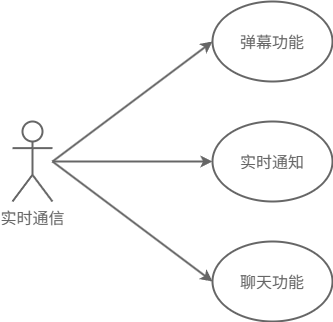
\includegraphics[width=0.5\textwidth]{实时通信.png}
    \caption{实时通信用例图}
    \label{实时通信用例图}
\end{figure}

弹幕功能极大地丰富了用户在视频观看过程中的互动体验,让用户能够在观看视频时实时分享自己的想法,增强用户之间的交流。当用户登录系统并进入视频播放页面后,可在专门设置的弹幕输入区域输入弹幕内容。完成输入后,用户点击“发送”按钮,系统会迅速将弹幕信息发送到服务器。服务器借助WebSocket技术,把该弹幕信息实时推送给所有正在观看同一视频的用户。这些弹幕会以动态形式在视频播放界面上显示出来,这样,每个用户在观看视频时,不仅能看到视频内容,还能实时浏览其他用户发送的弹幕,实现用户之间的即时互动,为视频观看增添乐趣。

实时通知功能确保系统能够及时向用户传达重要信息,如新消息提醒、系统公告等,使用户能够及时知晓与自身相关的事务和系统动态。系统在检测到需要推送的通知,如新消息到达、发布系统公告等情况时,会通过 WebSocket 将通知信息发送到服务器。服务器接收到通知信息后,会根据用户的相关信息,将通知实时推送给对应的用户。用户在登录系统后的界面上会收到通知提示,点击提示即可查看通知的具体内容,从而及时了解系统的最新动态和个人相关信息,保证用户与系统之间的信息同步。

聊天功能为用户搭建了一个实时交流的平台,方便用户与其他用户进行一对一或群组沟通,满足用户的社交需求。用户登录系统后进入聊天页面,在聊天页面中,用户可以选择想要聊天的对象,既可以是单个用户发起一对一聊天,也可以在群组聊天场景中选择相应群组。选定聊天对象后,用户在聊天框中输入想要发送的消息内容,输入完成后点击“发送”按钮,系统会将消息发送到服务器。服务器利用WebSocket技术,把消息实时推送给接收者。接收者在自己的聊天界面上会收到消息提醒,点击即可查看消息内容,实现用户之间高效、便捷的实时交流,促进用户之间的社交互动。

\subsection{非功能性需求分析}

系统非功能性需求指的是除功能性需求之外的特性,其中包括了软件质量、运行环境、外部接口等要求。非功能性需求从另外一个角度衡量一个系统是否符合用户需求,它要求我们在设计软件的时候不仅仅满足软件可用的要求,还要使软件易用,因此,非功能性需求与功能性需求同样重要\cite{RN08}。以下是本弹幕视频网站后端系统的非功能性需求:
\begin{enumerate}[label=(\arabic*)]
    \item 性能需求:作为一款视频网站,系统需要强大的高并发处理能力以确保大量用户同时使用的响应速度。除此之外为确保用户在高并发场景下仍然能够快速获取数据,实现流畅的操作,系统还应该优化网络传输机制以降低数据延迟。
    \item 可用性需求:系统应该具备高可用性,通过冗余设计对关键组件进行备份,确保当某个组件发生故障的时候系统能仍然能够持续正常与和运行。同时系统还要有完备的容错机制,能够自动检测和处理各种异常状况,减小异常状况发生时给用户带来的影响,保证服务的连续性。
    \item 安全性需求:据安全至关重要,系统需采用多种加密技术,对用户数据进行加密存储和传输,防止数据被窃取或篡改。在用户认证方面,要支持强身份验证机制,如多因素认证,确保只有授权用户能够访问系统。
    \item 可拓展性需求:系统应该具备良好的可拓展性以应付业务的增长与用户数量的增加,因此在设计之初就应该支持水平拓展和模块化设计。水平拓展通过增加节点提高了系统的存储与查询能力。模块化设计则便于日后的维护和拓展。
    \item 可维护性需求:系统的代码应具有良好的可读性,遵循统一的编程规范和代码风格,添加详细的注释,方便开发人员理解和修改代码。同时,建立完善的日志管理系统,记录系统运行过程中的关键事件、错误信息等。通过分析日志,开发人员可以快速定位问题,进行故障排查和修复,提高系统的维护效率。
\end{enumerate}

\newpage

\section{系统设计}

\subsection{系统架构设计}

\subsubsection{系统分层设计}

本系统采用基于SpringBoot与SpringCloud框架构建的微服务架构,系统架构图如\ref{系统架构图}所示。微服务架构的特点是将系统拆分成为了多个独立的服务,每个服务负责特定的功能,服务间通过轻量级通信机制(通常为HTTP REST API)进行交互\cite{EN03}。这种架构设计使系统具有高可用性、可拓展性和灵活性的特点。
\begin{figure}[hbt]
    \centering
    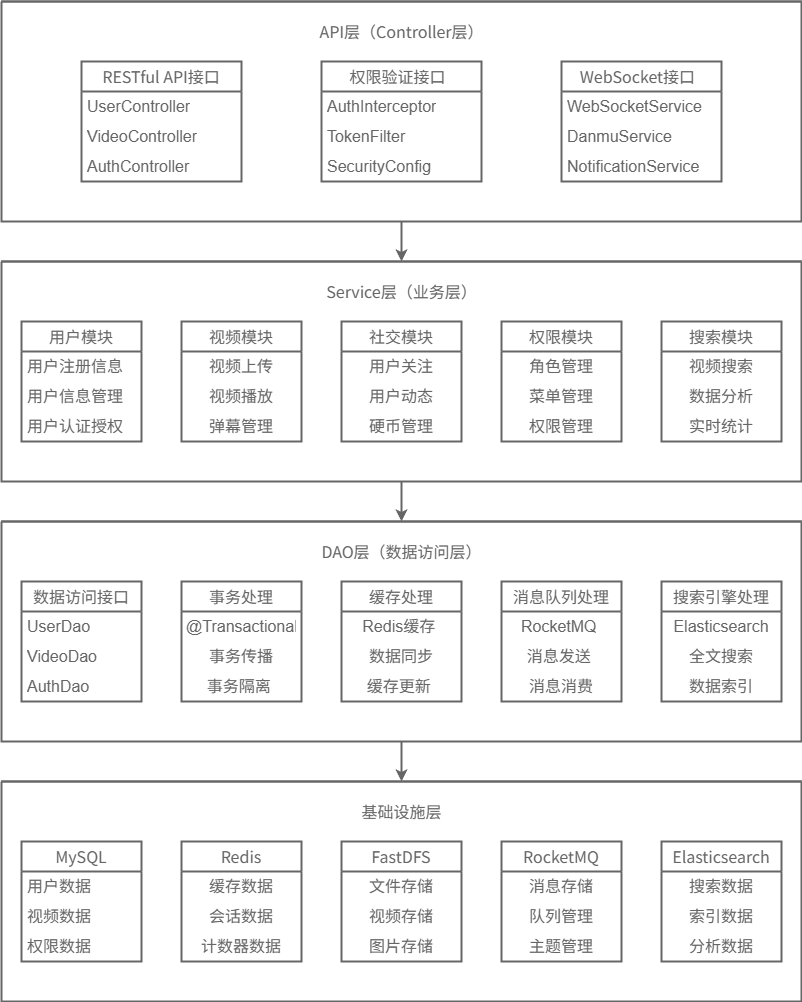
\includegraphics[width=0.5\textwidth]{系统架构.png}
    \caption{系统架构图}
    \label{系统架构图}
\end{figure}

在本系统的微服务下,请求在该架构下的传递过程如图\ref{请求传递过程}所示。

首先由客户端向本系统发送包含用户操作意图(如获取数据、执行某个功能)的HTTP或WebSocket请求,这个请求将被发送至API层。在API层对从接受的请求进行初步的验证和处理后,API层将会将请求转发给Service层,这一步处理是为了让接下来的Service层能够进行具体的业务处理。Service层在接受来自API层的请求后会根据业务需要进行逻辑处理,在处理完成后Service将会将数据操作的请求发送给DAO层。DAO层在接受数据操作请求后,会使用特定的数据访问技术和接口来操作基础设施层的数据存储。基础设施层在执行具体数据存储或读取操作后,再将结果返回给DAO层。DAO层在获取到数据操作结果后,结果将会被逐层向上处理包装,最终返还给客户端,完成了整个请求流程。
\begin{figure}[hbt]
    \centering
    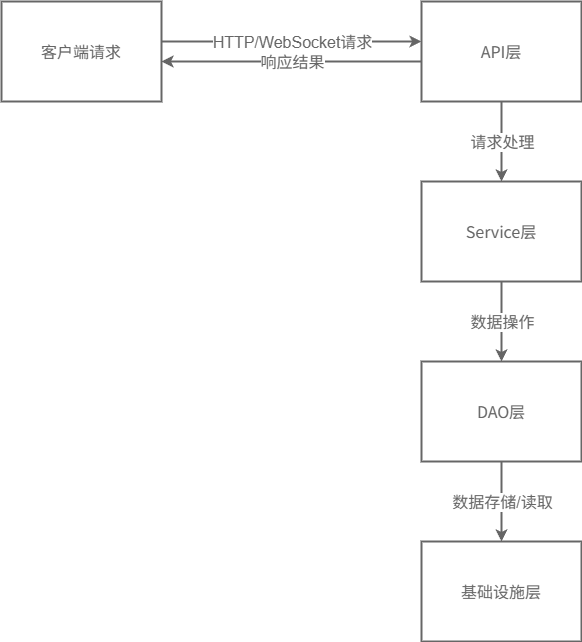
\includegraphics[width=0.5\textwidth]{请求传递.png}
    \caption{请求传递过程}
    \label{请求传递过程}
\end{figure}

\subsubsection{系统功能模块划分}

如图\ref{系统功能模块图}所示,本系统共分为用户管理、视频管理、社交互动、权限管理、搜索服务、消息通知、文件存储、系统监控共八大模块。
\begin{figure}[hbt]
    \centering
    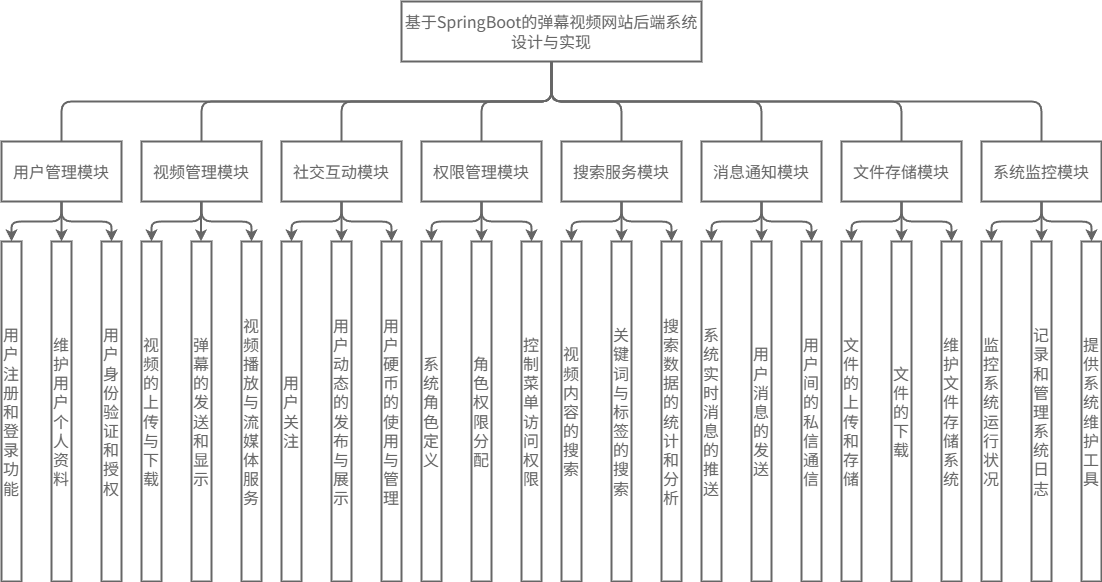
\includegraphics[width=1\textwidth]{系统功能模块.png}
    \caption{系统功能模块图}
    \label{系统功能模块图}
\end{figure}

垂直关系上,每个模块都遵循分层架构,实现架构层级由上而下的垂直调用。水平关系上,模块共享基础设施服务,模块间通过接口进行通信,模块解耦通过事件驱动实现。依赖关系上,权限模块为其他模块提供认证授权服务,文件存储模块为视频模块提供存储服务,消息模块为其他模块提供通知服务。

\subsection{系统数据库设计}

\subsubsection{数据库概念结构设计}

开发者在充分掌握用户需求的基础上,边可以开始展开对数据库的概念结构设计,即将用户相对抽象的需求进行一定的具象化,使之成为能够指引后续设计过程的概念模型\cite{RN09}。本弹幕视频网站系统的数据库所使用的数据库类型是MySQL数据库,数据库实体关系图如\ref{实体关系图}。

\begin{figure}[hbt]
    \centering
    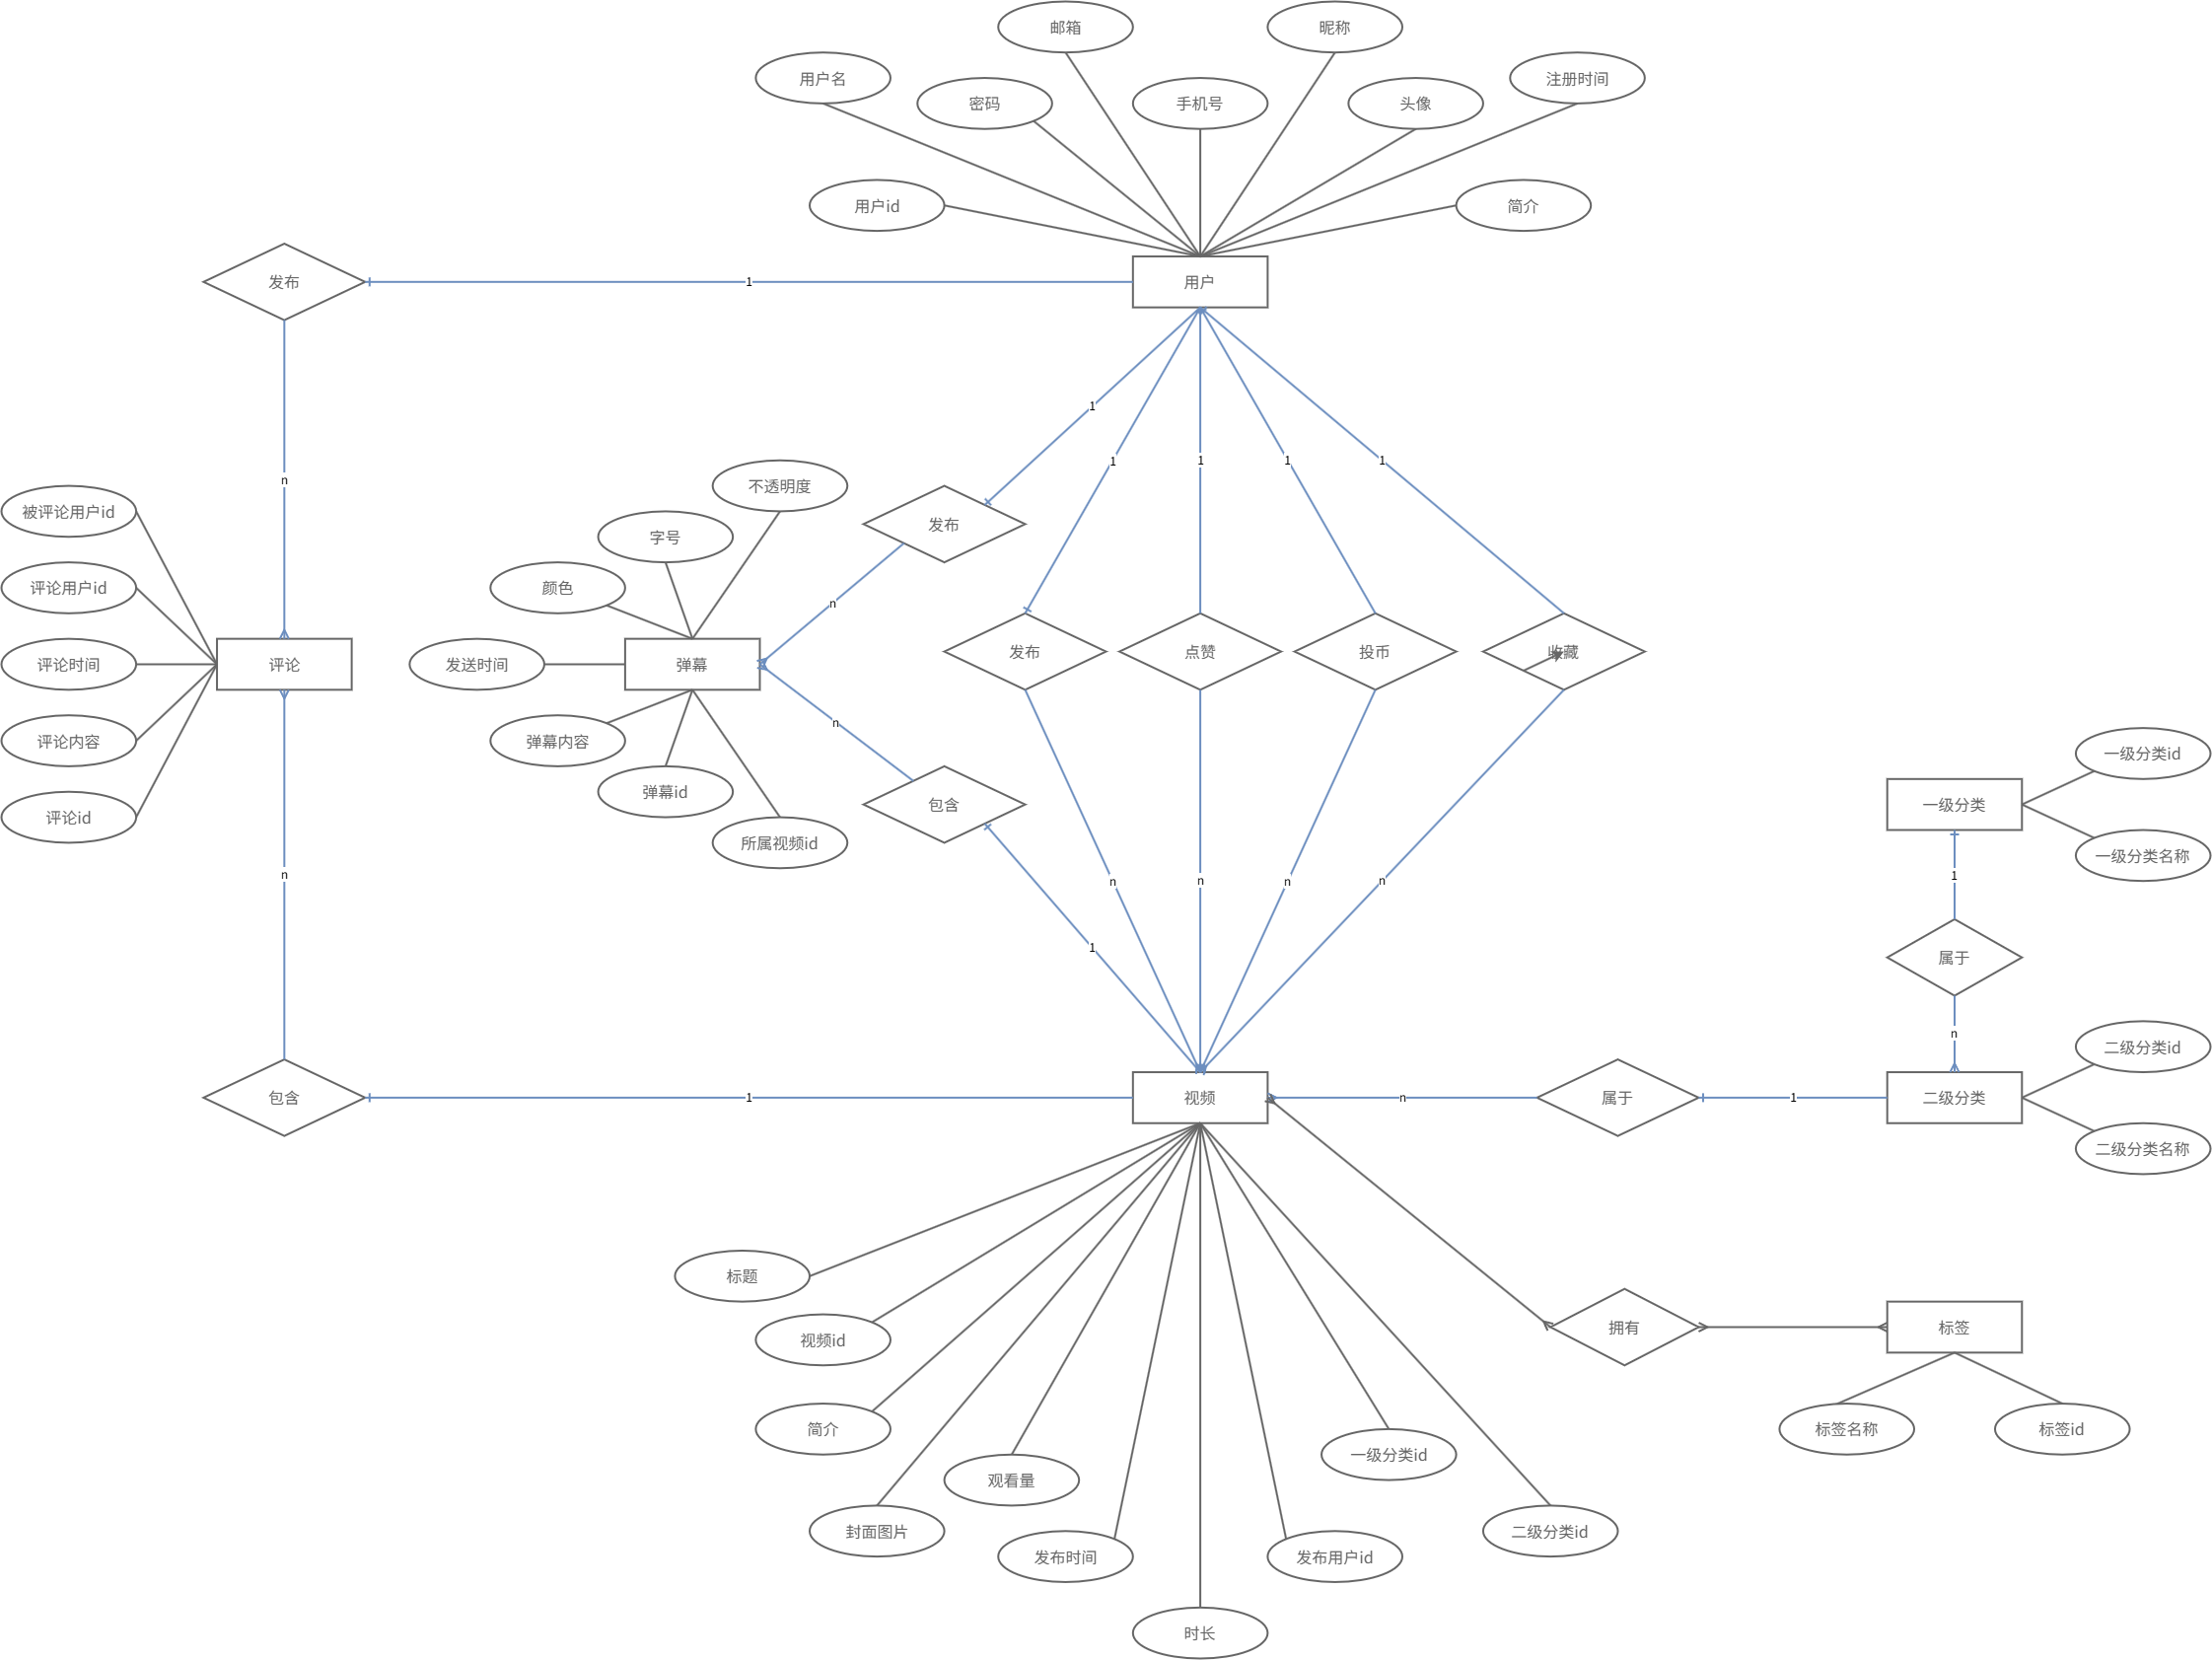
\includegraphics[width=1\textwidth]{实体关系.png}
    \caption{实体关系图}
    \label{实体关系图}
\end{figure}

根据实体关系图\ref{实体关系图}可以知道,数据库中的实体主要包括用户User、视频Video、弹幕Danmu、评论Comment、一级分类Category1、二级分类Category2以及标签Tag。对于本数据库中的用户、视频、弹幕、评论四个主要实体的具体描述属性如下:

\begin{enumerate}[label=(\arabic*)]
    \item 用户实体负责储存系统中的所有用户信息,包括用户id、用户名、昵称、头像、邮箱、手机号、密码、注册时间、简介。用户实体图如图\ref{用户实体图}所示。
    \begin{figure}[hbt]
        \centering
        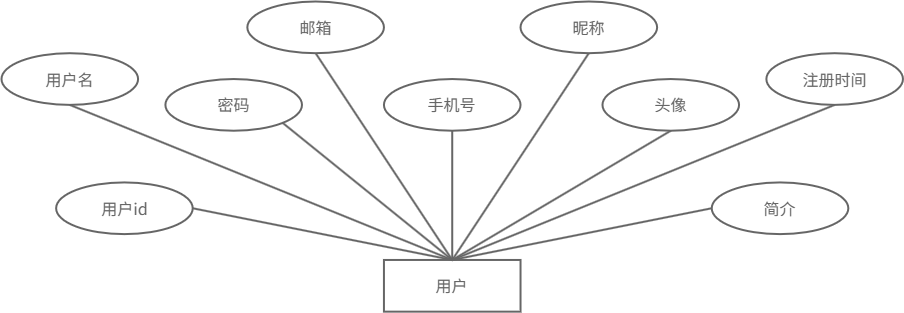
\includegraphics[width=0.5\textwidth]{用户实体.png}
        \caption{用户实体图}
        \label{用户实体图}
    \end{figure}
    \item 视频实体负责存储系统中的所有的视频信息,包括标题、视频id、简介、封面图片、观看量、发布时间、市场、发布用户id、一级分类id、二级分类id 。视频实体图如图\ref{视频实体图}所示。
    \begin{figure}[hbt]
        \centering
        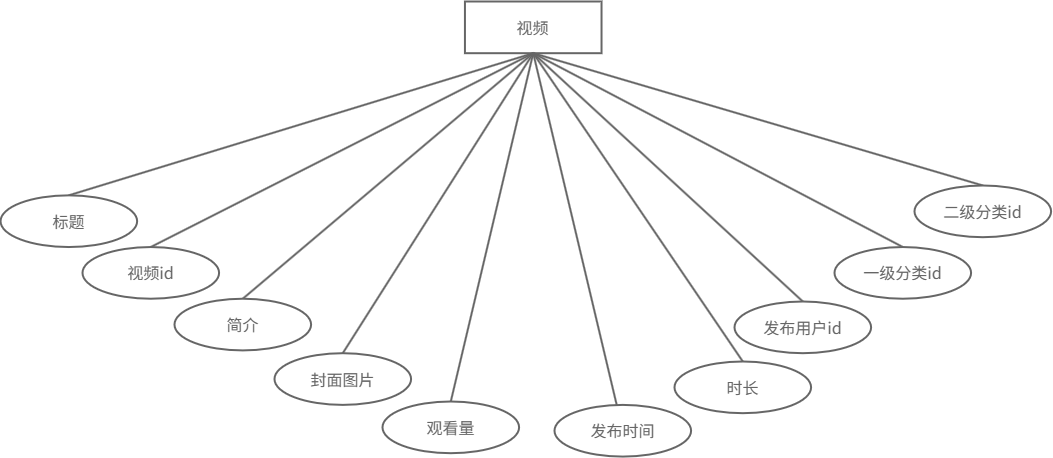
\includegraphics[width=0.5\textwidth]{视频实体.png}
        \caption{视频实体图}
        \label{视频实体图}
    \end{figure}
    \item 弹幕实体负责存储系统中的弹幕信息,包括弹幕内容、不透明度、颜色、字号、发送时间、弹幕id、所属视频id。弹幕实体图如图\ref{弹幕实体图}所示。
    \begin{figure}[hbt]
        \centering
        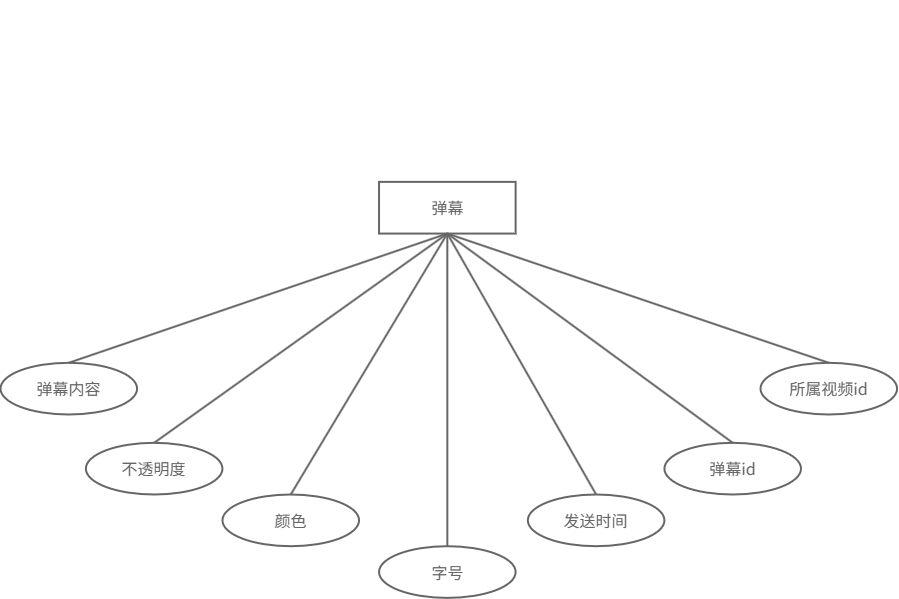
\includegraphics[width=0.5\textwidth]{弹幕实体.png}
        \caption{弹幕实体图}
        \label{弹幕实体图}
    \end{figure}
    \item 评论实体负责储存系统中的评论信息,包括评论用户id、评论时间、被评论用户id、评论内容、评论id。评论实体图如图\ref{评论实体图}所示
    \begin{figure}[hbt]
        \centering
        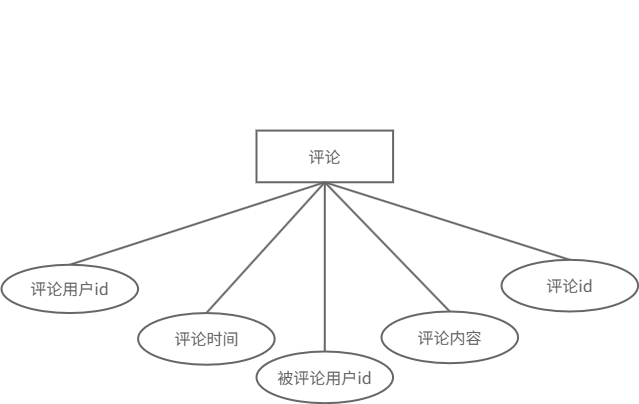
\includegraphics[width=0.5\textwidth]{评论实体.png}
        \caption{评论实体图}
        \label{评论实体图}
    \end{figure}

\end{enumerate}

其中用户与视频、用户与评论、用户与弹幕、视频与评论、视频与弹幕、一级分类与二级分类均属于一对多的关系。视频与二级分类属于多对一的关系。视频与标签属于多对多的关系。

\subsubsection{数据库逻辑结构设计}

基本表是数据的存储过程建立的基础,因此在数据库设计时应首先建好表\cite{RN10}。根据弹幕视频网站后端系统的业务需求分析以及数据库设计原则,将基本实体图转换成MySQL支持的数据模型相符合的逻辑结构,采用合适的数据类型,完成系统数据表的设计。

本数据库名称叫做imooc-bilibili,数据库中包括4张数据表:用户相关表、视频相关表、权限相关表以及其他功能表。每个表都包含主键id、创建时间creatTime、更新时间updatetime(部分表)和相关外键关联字段。

以下列出主要的数据表:
\begin{enumerate}[label=(\arabic*)]
    \item 用户相关表
    
    用户相关表主要存储用户相关信息,如下表\ref{用户相关表}所示。
    \begin{table}[htb]
        \centering
        \caption{用户相关表}
        \label{用户相关表}
        
        \begin{tabular}{|l|l|l|}
        \hline
        \textbf{表名} & \textbf{说明} & \textbf{主要字段} \\
        \hline
        \makecell{t\_user} & \makecell{用户表} & \makecell{id, phone, email, password, salt, \\createTime,  updateTime} \\
        \hline
        \makecell{t\_user\_info} & \makecell{用户基本信息表} & \makecell{id, userId, nick, avatar, sign, gender, birth, \\createTime, updateTime} \\
        \hline
        \makecell{t\_user\_following} & \makecell{用户关注表} & \makecell{id, userId, followingId, groupId, \\createTime} \\
        \hline
        \makecell{t\_user\_moments} & \makecell{用户动态表} & \makecell{id, userId, type, contentId, \\createTime, updateTime} \\
        \hline
        \makecell{t\_user\_coin} & \makecell{用户硬币表} & \makecell{id, userId, amount, \\createTime, updateTime} \\
        \hline
        \makecell{t\_user\_role} & \makecell{用户角色关联表} & \makecell{id, userId, roleId, createTime} \\
        \hline
        \makecell{t\_refresh\_token} & \makecell{刷新令牌记录表} & \makecell{id, userId, refreshToken, \\createTime} \\
        \hline
    \end{tabular}
    \end{table}

    \item 视频相关表
    
    视频相关表主要存储视频相关信息,如下表\ref{视频相关表}所示。
    \begin{table}[htb]
        \centering
        \caption{视频相关表}
        \label{视频相关表}
        \begin{tabular}{|l|l|l|}
        \hline
        \textbf{表名} & \textbf{说明} & \textbf{主要字段} \\
        \hline
        \makecell{t\_video} & \makecell{视频投稿记录表} & \makecell{id, userId, url, thumbnail, title, type, duration,\\ area, description, createTime, updateTime} \\
        \hline
        \makecell{t\_video\_comment} & \makecell{视频评论表 }& \makecell{id, videoId, userId, comment, replyUserId, \\rootId, createTime, updateTime} \\
        \hline
        \makecell{t\_video\_coin} & \makecell{视频硬币表} & \makecell{id, userId, videoId, amount, \\createTime, updateTime} \\
        \hline
        \makecell{t\_video\_collection} & \makecell{视频收藏记录表} & \makecell{id, videoId, \\userId, groupId, createTime} \\
        \hline
        \makecell{t\_video\_like }& \makecell{视频点赞记录表} & \makecell{id, userId, videoId, createTime} \\
        \hline
        \makecell{t\_video\_tag} & \makecell{视频标签关联表} & \makecell{id, videoId, tagId, createTime} \\
        \hline
        \makecell{t\_video\_view} & \makecell{视频观看记录表} & \makecell{id, videoId, userId, clientId, \\ip, createTime} \\
        \hline
        \makecell{t\_video\_binary\_picture} & \makecell{视频二值图记录表} & \makecell{id, videoId, frameNo, url, \\videoTimestamp, createTime} \\
        \hline
        \makecell{t\_video\_operation} & \makecell{视频操作表} & \makecell{id, userId, videoId, \\operationType, createTime} \\
        \hline
        \end{tabular}
        \end{table}
    
    \item 权限相关表

    权限相关表主要储存权限控制的相关信息,如下表\ref{权限相关表}所示。
    \begin{table}[h]
        \centering
        \caption{权限相关表}
        \label{权限相关表}
        \begin{tabular}{|l|l|l|}
        \hline
        \textbf{表名} & \textbf{说明} & \textbf{主要字段} \\
        \hline
        \makecell{t\_auth\_role }& \makecell{权限控制-角色表} & \makecell{id, name, code, \\createTime, updateTime} \\
        \hline
        \makecell{t\_auth\_menu} & \makecell{权限控制-\\页面访问表} & \makecell{id, name, code, \\createTime, updateTime }\\
        \hline
        \makecell{t\_auth\_\\element\_operation} & \makecell{权限控制-\\页面元素操作表} & \makecell{id, elementName, elementCode, \\operationType, createTime, updateTime }\\
        \hline
        \makecell{t\_auth\_role\_menu} & \makecell{权限控制-\\角色页面菜单关联表} & \makecell{id, roleId, menuId, createTime }\\
        \hline
        \makecell{t\_auth\_role\_\\element\_operation} & \makecell{权限控制-\\角色与元素操作关联表 }& \makecell{id, roleId, elementOperationId, \\createTime}\\
        \hline
        \end{tabular}
        \end{table}
    
    \item 其他功能表
    
    其他功能表主要存储剩余功能的相关信息,如下表\ref{其他功能表}所示。
    \begin{table}[h]
        \centering
        \caption{其他功能表}
        \label{其他功能表}
        \begin{tabular}{|l|l|l|}
        \hline
        \textbf{表名} & \textbf{说明} & \textbf{主要字段} \\
        \hline
        \makecell{t\_danmu} & \makecell{弹幕记录表} & \makecell{id, userId, videoId, content, danmuTime, createTime} \\
        \hline
        \makecell{t\_file} & \makecell{文件表} & \makecell{id, url, type, md5, createTime} \\
        \hline
        \makecell{t\_following\_group} & \makecell{用户关注分组表} & \makecell{id, userId, name, type, createTime, updateTime} \\
        \hline
        \makecell{t\_collection\_group} & \makecell{收藏分组表} & \makecell{id, userId, name, type, createTime, updateTime} \\
        \hline
        \makecell{t\_tag} & \makecell{标签表} & \makecell{id, name, createTime} \\
        \hline
        \makecell{t\_content} & \makecell{动态内容表} & \makecell{id, contentDetail, createTime} \\
        \hline
        \end{tabular}
        \end{table}
\end{enumerate}
\newpage

\section{系统实现}

\subsection{技术栈、开发环境与开发工具介绍}

\subsubsection{开发环境}

该项目的开发环境整合了多种系统工具与中间件服务。系统环境上,以Windows 10(版本 10.0.22631)为操作系统,搭配Java8作为开发语言环境,利用Maven进行项目构建,通过Git实现版本控制。中间件方面,MySQL8.0负责数据库服务,用于存储结构化数据;Redis提供缓存服务,加速数据读取;RocketMQ作为消息队列服务,处理异步任务;Elasticsearch实现搜索服务,满足数据检索需求;FastDFS承担文件存储服务,管理非结构化文件。这些系统工具和中间件协同工作,为项目开发、运行提供了稳定且高效的环境基础。

\subsubsection{技术栈}

在后端框架层面,因SpringBoot快速开发、自动配置等的特性\ref{SpirngBoot特性}能够减少大量繁琐的配置工作,极大提升了开发效率,所以选定SpringBoot2.5.1为基础框架。在此之上,引入SpringCloud微服务框架,在该框架下,本系统借助Netflix Eureka实现服务注册与发现,实现了各个微服务之间能够相互识别与通信,保障系统的动态管理与扩展;OpenFeign用于服务间通信,提供了声明式的 Web 服务客户端,简化了服务调用过程;Hystrix实现服务熔断机制,当某个服务出现故障时,能及时切断请求,防止故障扩散,确保系统整体的稳定性。

数据存储方面,选用MySQL8.0作为关系型数据库,负责存储结构化数据,如用户信息、视频元数据等,其强大的数据处理和事务管理能力为系统提供了可靠的数据支持。Redis作为缓存数据库,将频繁访问的数据存储在内存中,加速数据读取,减轻数据库压力。Elasticsearch作为搜索引擎,实现高效的视频搜索功能,支持复杂的全文检索等操作。FastDFS分布式文件存储则用于存储视频文件等大量非结构化数据,保证文件存储的高可靠性和可扩展性。

在消息队列方面选用了RocketMQ它承担了异步处理的任务,在系统发起处理视频上传、弹幕发送等异步任务时,它能够起到削峰填谷、解耦应用等作用。能够提升系统的整体性能和响应速度。

其他技术中,MyBatis作为ORM框架,方便地实现了Java对象与数据库表之间的映射,简化了数据持久化操作。WebSocket实现实时通信,为弹幕功能提供技术支撑,使用户能实时发送和接收弹幕消息。JWT用于用户认证,通过生成和验证JSON Web Token,确保只有合法用户能够访问系统资源,保障系统安全。Mahout作为推荐引擎,分析用户行为数据,为用户推荐个性化的视频内容。JavaCV则专注于视频处理,例如对上传的视频进行格式转换、剪辑等操作,满足多样化的视频处理需求。

\subsubsection{开发工具}

本次系统开发选择Intelli IDEA作为主要开发工具,它集成了众多实用功能。通过搭配以下多个关键插件使用,能够实现简化代码编写、提升开发效率的目的,进一步增强了开发能力。
\begin{enumerate}[label=(\arabic*)]
    \item Lombok:通过注解自动生成常用代码,减少冗余代码量,简化了Java对象的代码编写。
    \item MyBatisX:顾名思义为MyBatis框架开发提供便利,支持XML与注解两种开发方式,能够快速生成SQL语句、映射文件等。
    \item SrpingBoot Assistant:专门针对SpringBoot项目,提供快速创建项目、自动配置等的功能,加速应用开发进程。
    \item Maven Helper:优化了Maven项目管理,方便管理项目依赖、解决依赖冲突等问题。
\end{enumerate}

除IDEA外,本系统还使用了Cursor编辑器作为辅助编辑器。它是一款具备AI辅助编程功能的编辑器,其AI代码补全功能能够根据上下文推测并补全代码,提高代码编写错误;代码重构的功能可以对现有代码优化,提升代码的可读性和可维护性。同时,智能提示功能可以实时为开发者提供代码建议,代码分析功能则能够检测代码中像语法错误这样的潜在问题,助力开发者编写出高质量的代码。

此外,我们还有几种不同的工具搭配使用来保障项目的顺利开发。Postman用于API测试,能方便地发送各种HTTP请求,对开发的API接口进行功能测试、性能测试等,确保API的正确性和稳定性。Navicat作为专业的数据库管理工具,方便管理MySQL等数据库,可进行数据库设计、数据操作、备份恢复等工作。Redis Desktop Manager 专门用于Redis数据库管理,以图形化界面展示 Redis 中的数据,方便进行数据查看、修改、删除等操作。Git作为版本控制工具,结合Maven的项目依赖管理功能,实现对项目代码和依赖的有效管理,方便团队协作开发,追踪代码变更历史,管理项目版本 。Github Desktop作为GitHub为Git开发的图形化工具,它大大简化了Git与Github的使用流程,尤其适合不熟悉命令行操作的开发者。

\subsection{核心架构搭建}

本系统主要使用基于SpringBoot框架的微服务架构搭建而成的Maven项目工程,从主架构图\ref{主架构图}
可知,本系统在由API模块、服务模块和数据访问模块三个子模块构成,这三个子模块的详细结构如图\ref{子模块结构}(以API模块为例)。
\begin{figure}[hbt]
    \centering
    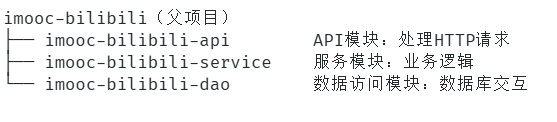
\includegraphics[width=0.5\textwidth]{主架构.png}
    \caption{主架构图}
    \label{主架构图}
\end{figure}

\begin{figure}[hbt]
    \centering
    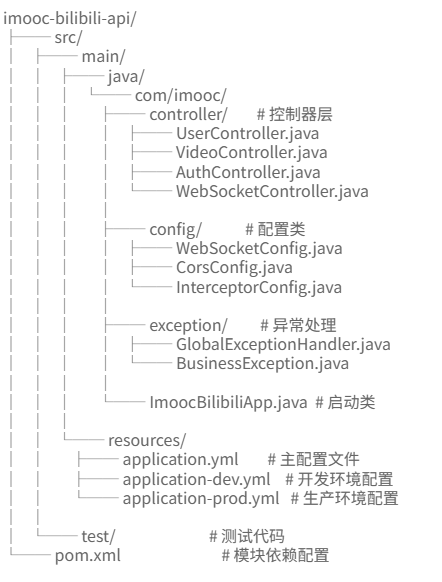
\includegraphics[width=0.5\textwidth]{子模块.png}
    \caption{子模块结构}
    \label{子模块结构}
\end{figure}

在父项目的目录下的pom.xml文件,它是Maven项目的核心配置文件。首先它包含着项目的基本信息,这些信息用作唯一标识一个Maven项目;其次POM文件还可以管理项目的依赖关系,通过<dependencies>标签定义项目所需要的库,例如图\ref{POM依赖管理}

\begin{figure}[hbt]
    \centering
    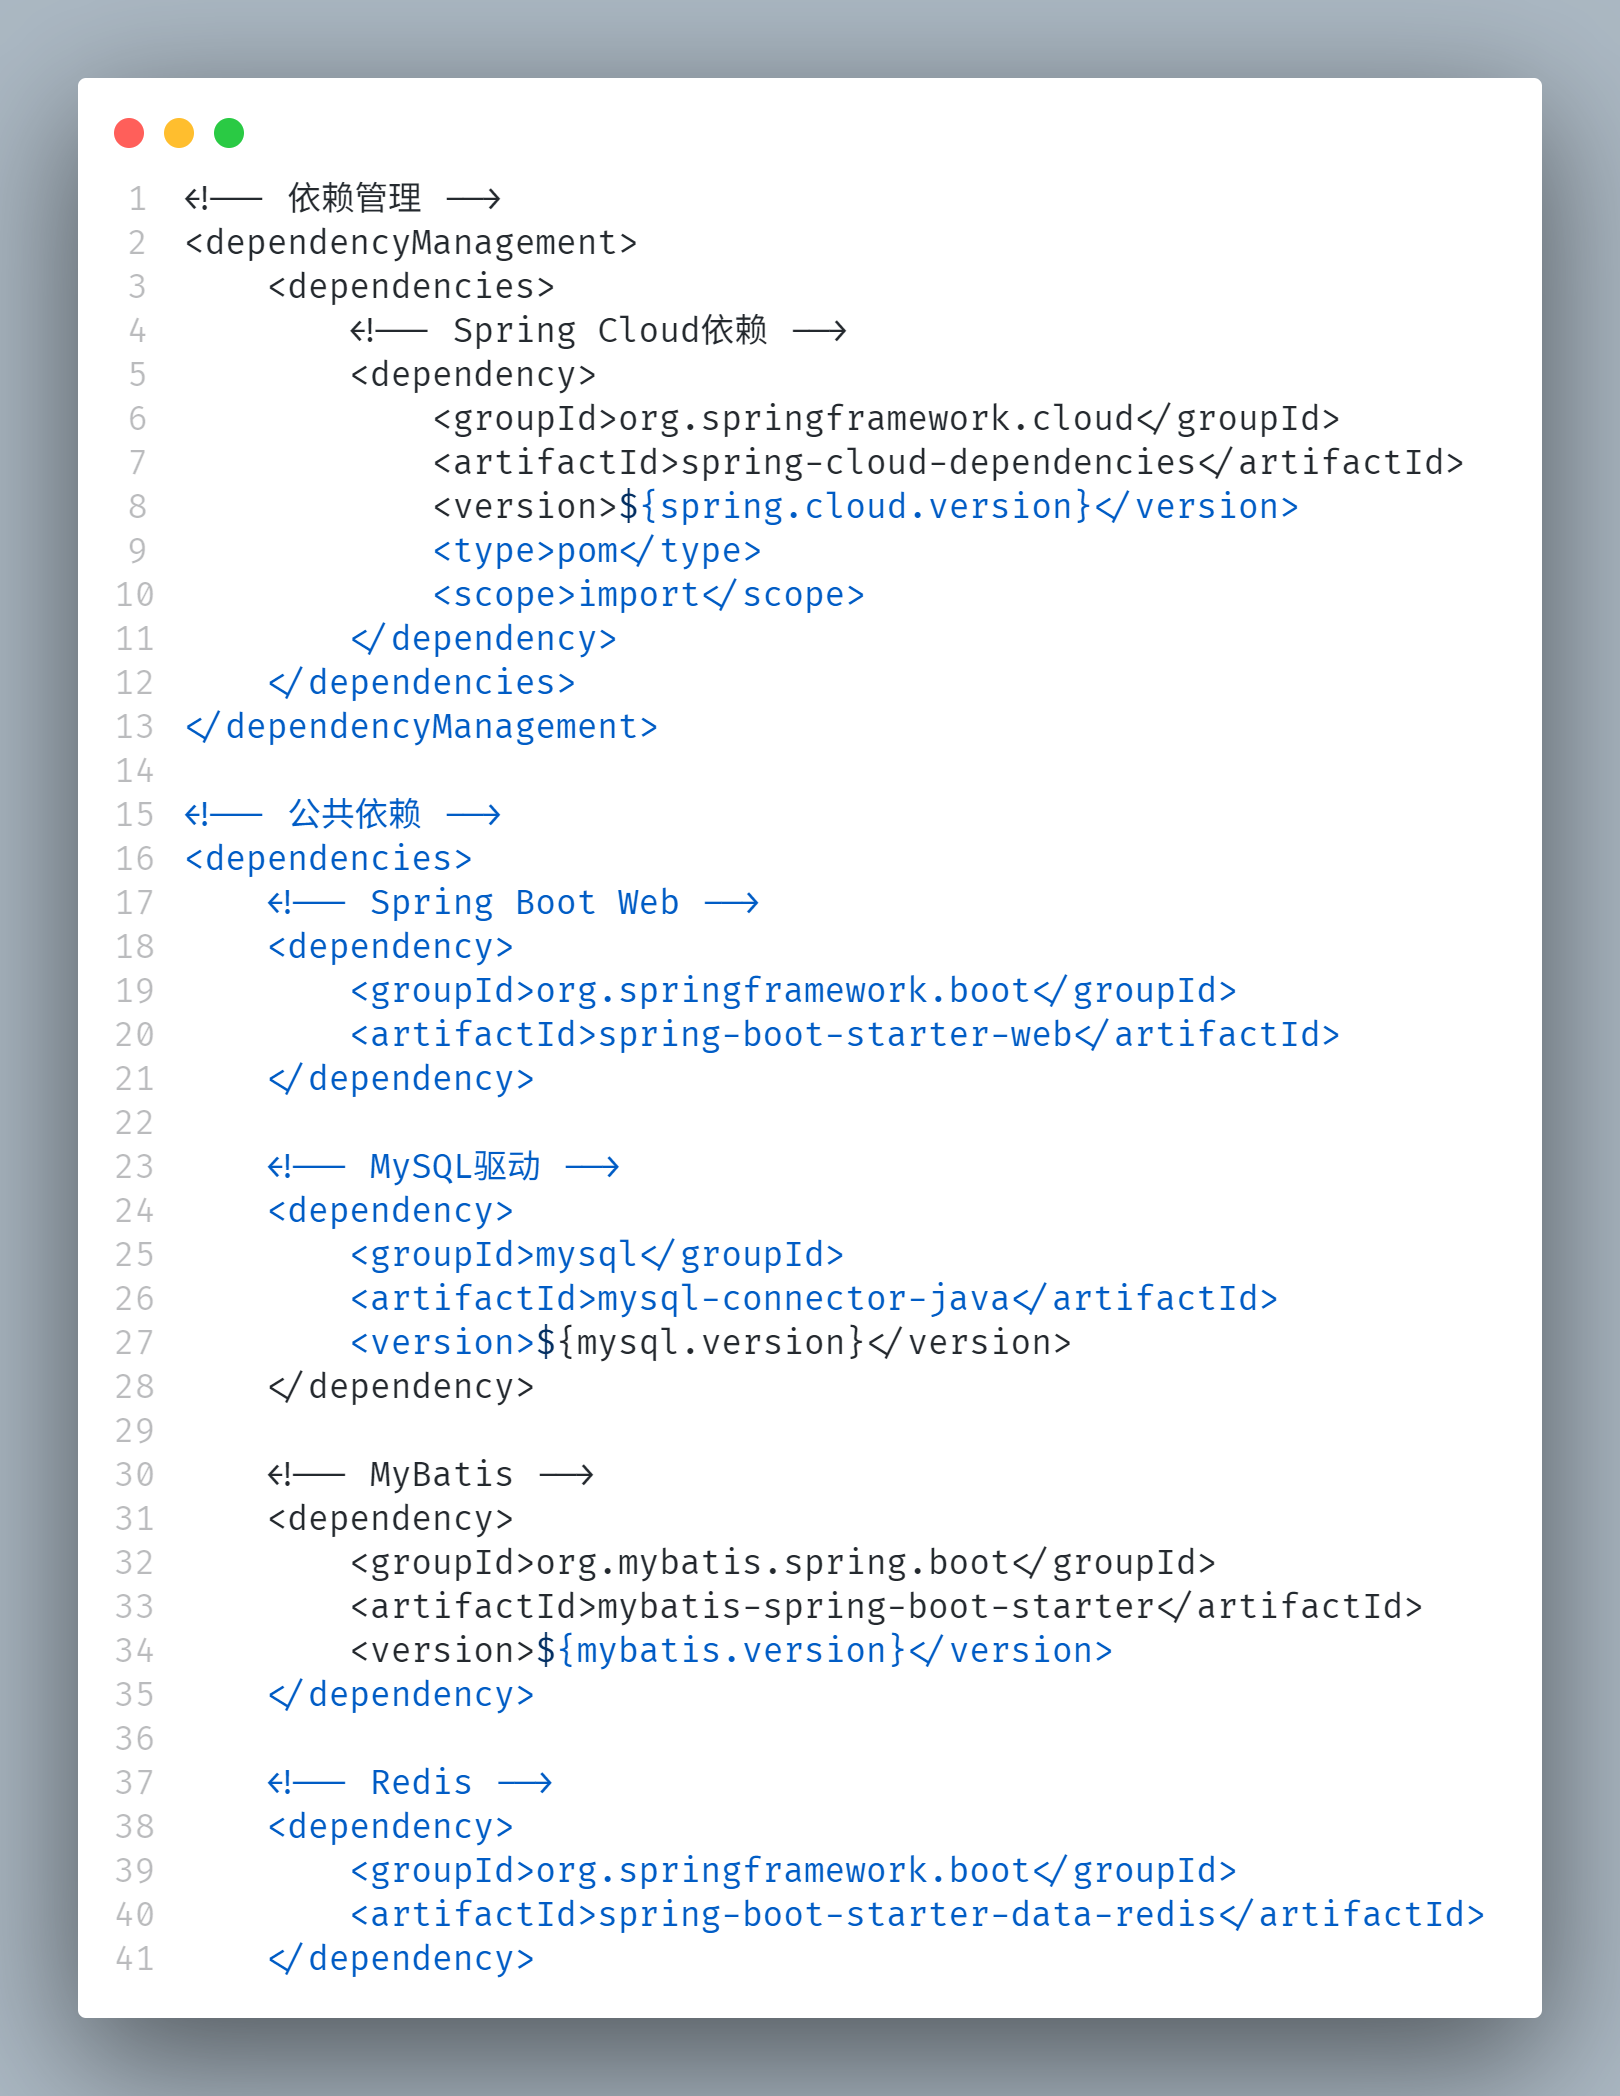
\includegraphics[width=1.0\textwidth]{POM依赖管理.png}
    \caption{POM依赖管理}
    \label{POM依赖管理}
\end{figure}

\subsection{关键模块实现}

\subsubsection{用户模块}

在系统的用户服务模块图\ref{用户模块伪代码}中,UserServiceImpl类承担着核心的业务逻辑处理工作,它实现了UserService接口,借助@Service注解被Spring容器识别为服务组件。

\begin{figure}[hbt]
    \centering
    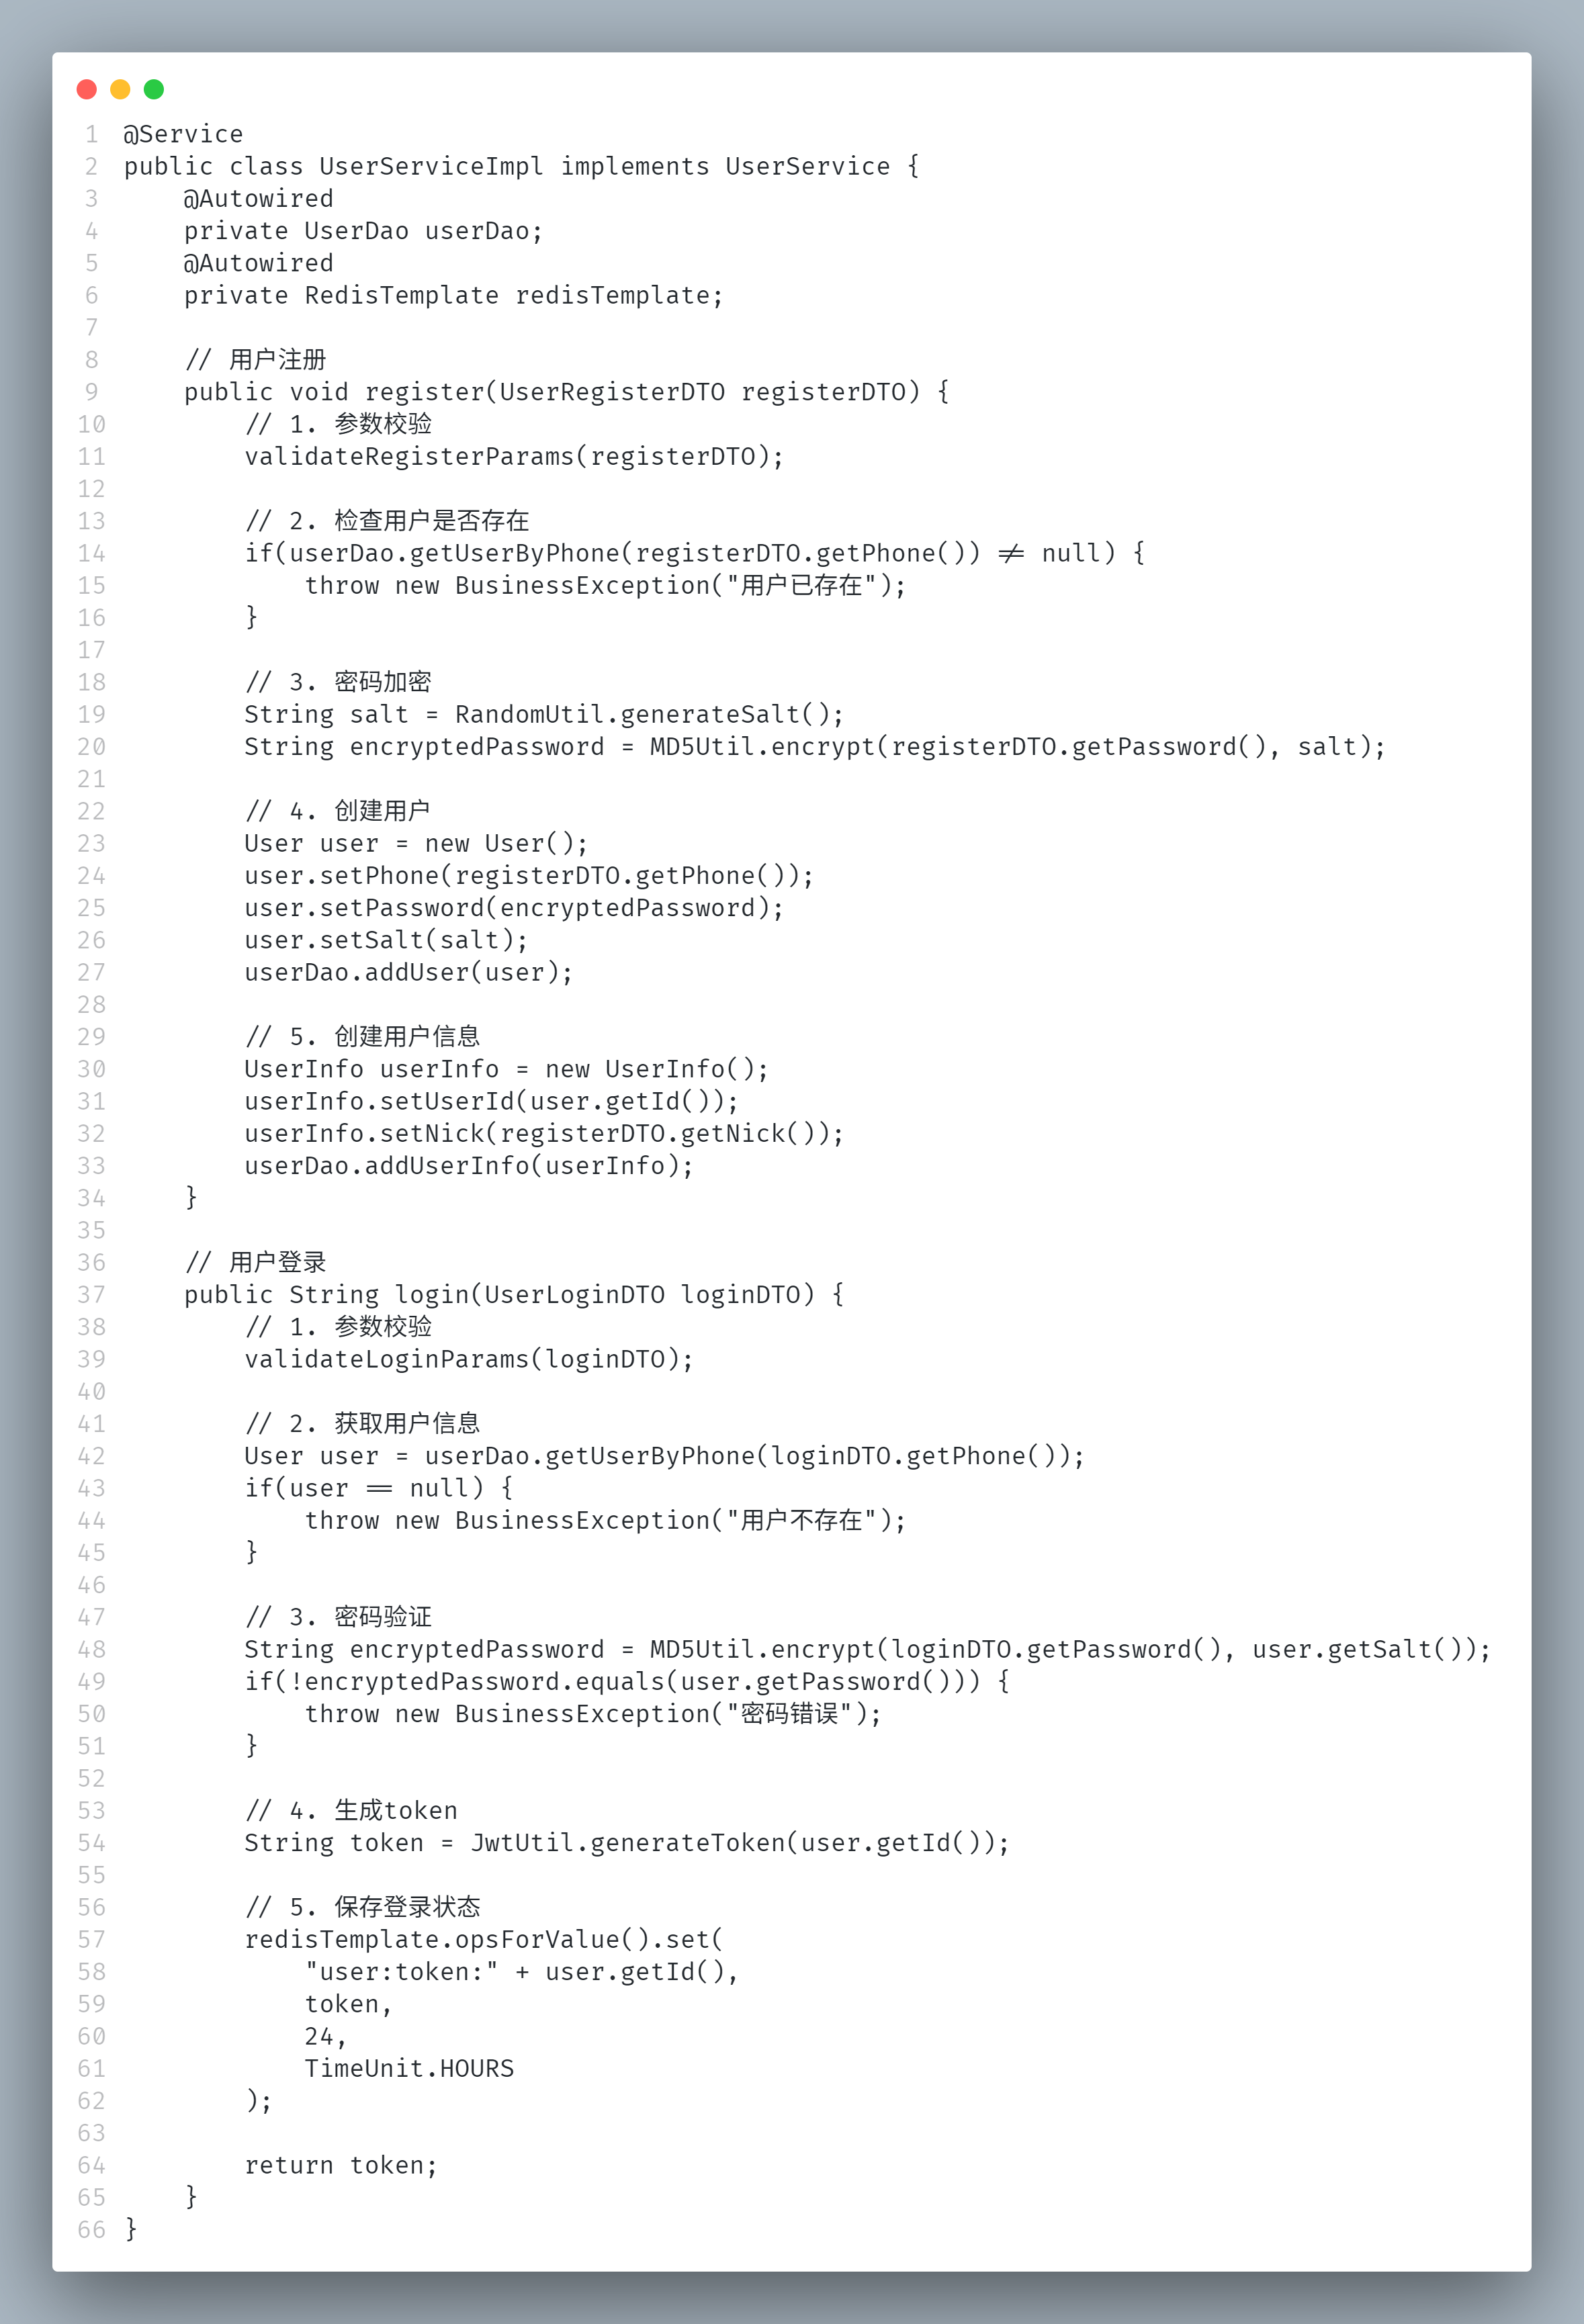
\includegraphics[width=0.75\textwidth]{用户模块.png}
    \caption{用户模块伪代码}
    \label{用户模块伪代码}
\end{figure}


用户注册功能当用户发起注册请求时,系统会调用 register 方法。具体处理流程如下:
\begin{enumerate}[label=(\arabic*)]
    \item 参数校验:对用户提交的注册信息进行初步的合法性检查,确保数据的完整性和准确性。
    \item 用户存在性检查:通过UserDao访问数据库,依据用户提供的手机号码查询是否已有该用户存在。若存在,则抛出BusinessException异常,提示 “用户已存在”。
    \item 密码加密处理:为保证用户密码的安全性,系统会生成一个随机的盐值,然后使用MD5加密算法结合盐值对用户输入的密码进行加密。
    \item 用户记录创建:创建一个User对象,将加密后的密码和盐值存储其中,并通过UserDao将用户信息持久化到数据库。
    \item 用户信息创建:接着创建一个UserInfo对象,将用户的昵称等信息存储其中,并与用户ID 关联,最后同样通过 UserDao 将用户信息保存到数据库。

\end{enumerate}

用户登录功能当用户尝试登录系统时,系统会调用login方法。具体处理步骤如下:
\begin{enumerate}[label=(\arabic*)]
    \item 参数校验:对用户提交的登录信息进行基本的格式和完整性检查。
    \item 用户信息获取:通过UserDao根据用户输入的手机号码从数据库中获取对应的用户信息。若未找到该用户,则抛出BusinessException异常,提示 “用户不存在”。
    \item 密码验证:使用相同的MD5加密算法和数据库中存储的盐值对用户输入的密码进行加密,然后将加密后的密码与数据库中存储的密码进行比对。若不一致,则抛出BusinessException异常,提示 “密码错误”。
    \item Token 生成:若密码验证通过,系统会使用JWT(JSON Web Token)工具为用户生成一个唯一的令牌,用于标识用户的身份。
    \item 登录状态保存:将生成的令牌存储到Redis缓存中,并设置 24 小时的有效期,以此来保存用户的登录状态。最后,将生成的令牌返回给用户,用于后续的身份验证和访问授权。

\end{enumerate}

通过上述功能的实现,该用户服务模块为系统提供了安全、可靠的用户注册和登录服务,有效地保障了用户信息的安全和系统的正常运行。

\subsubsection{视频模块}

如图\ref{视频模块伪代码}在视频模块的服务实现中,VideoServiceImpl类发挥着关键作用。该类通过@Service注解被 Spring 容器识别为服务组件,实现了VideoService接口,为视频的上传和播放功能提供了具体的业务逻辑处理。
\begin{figure}[hbt]
    \centering
    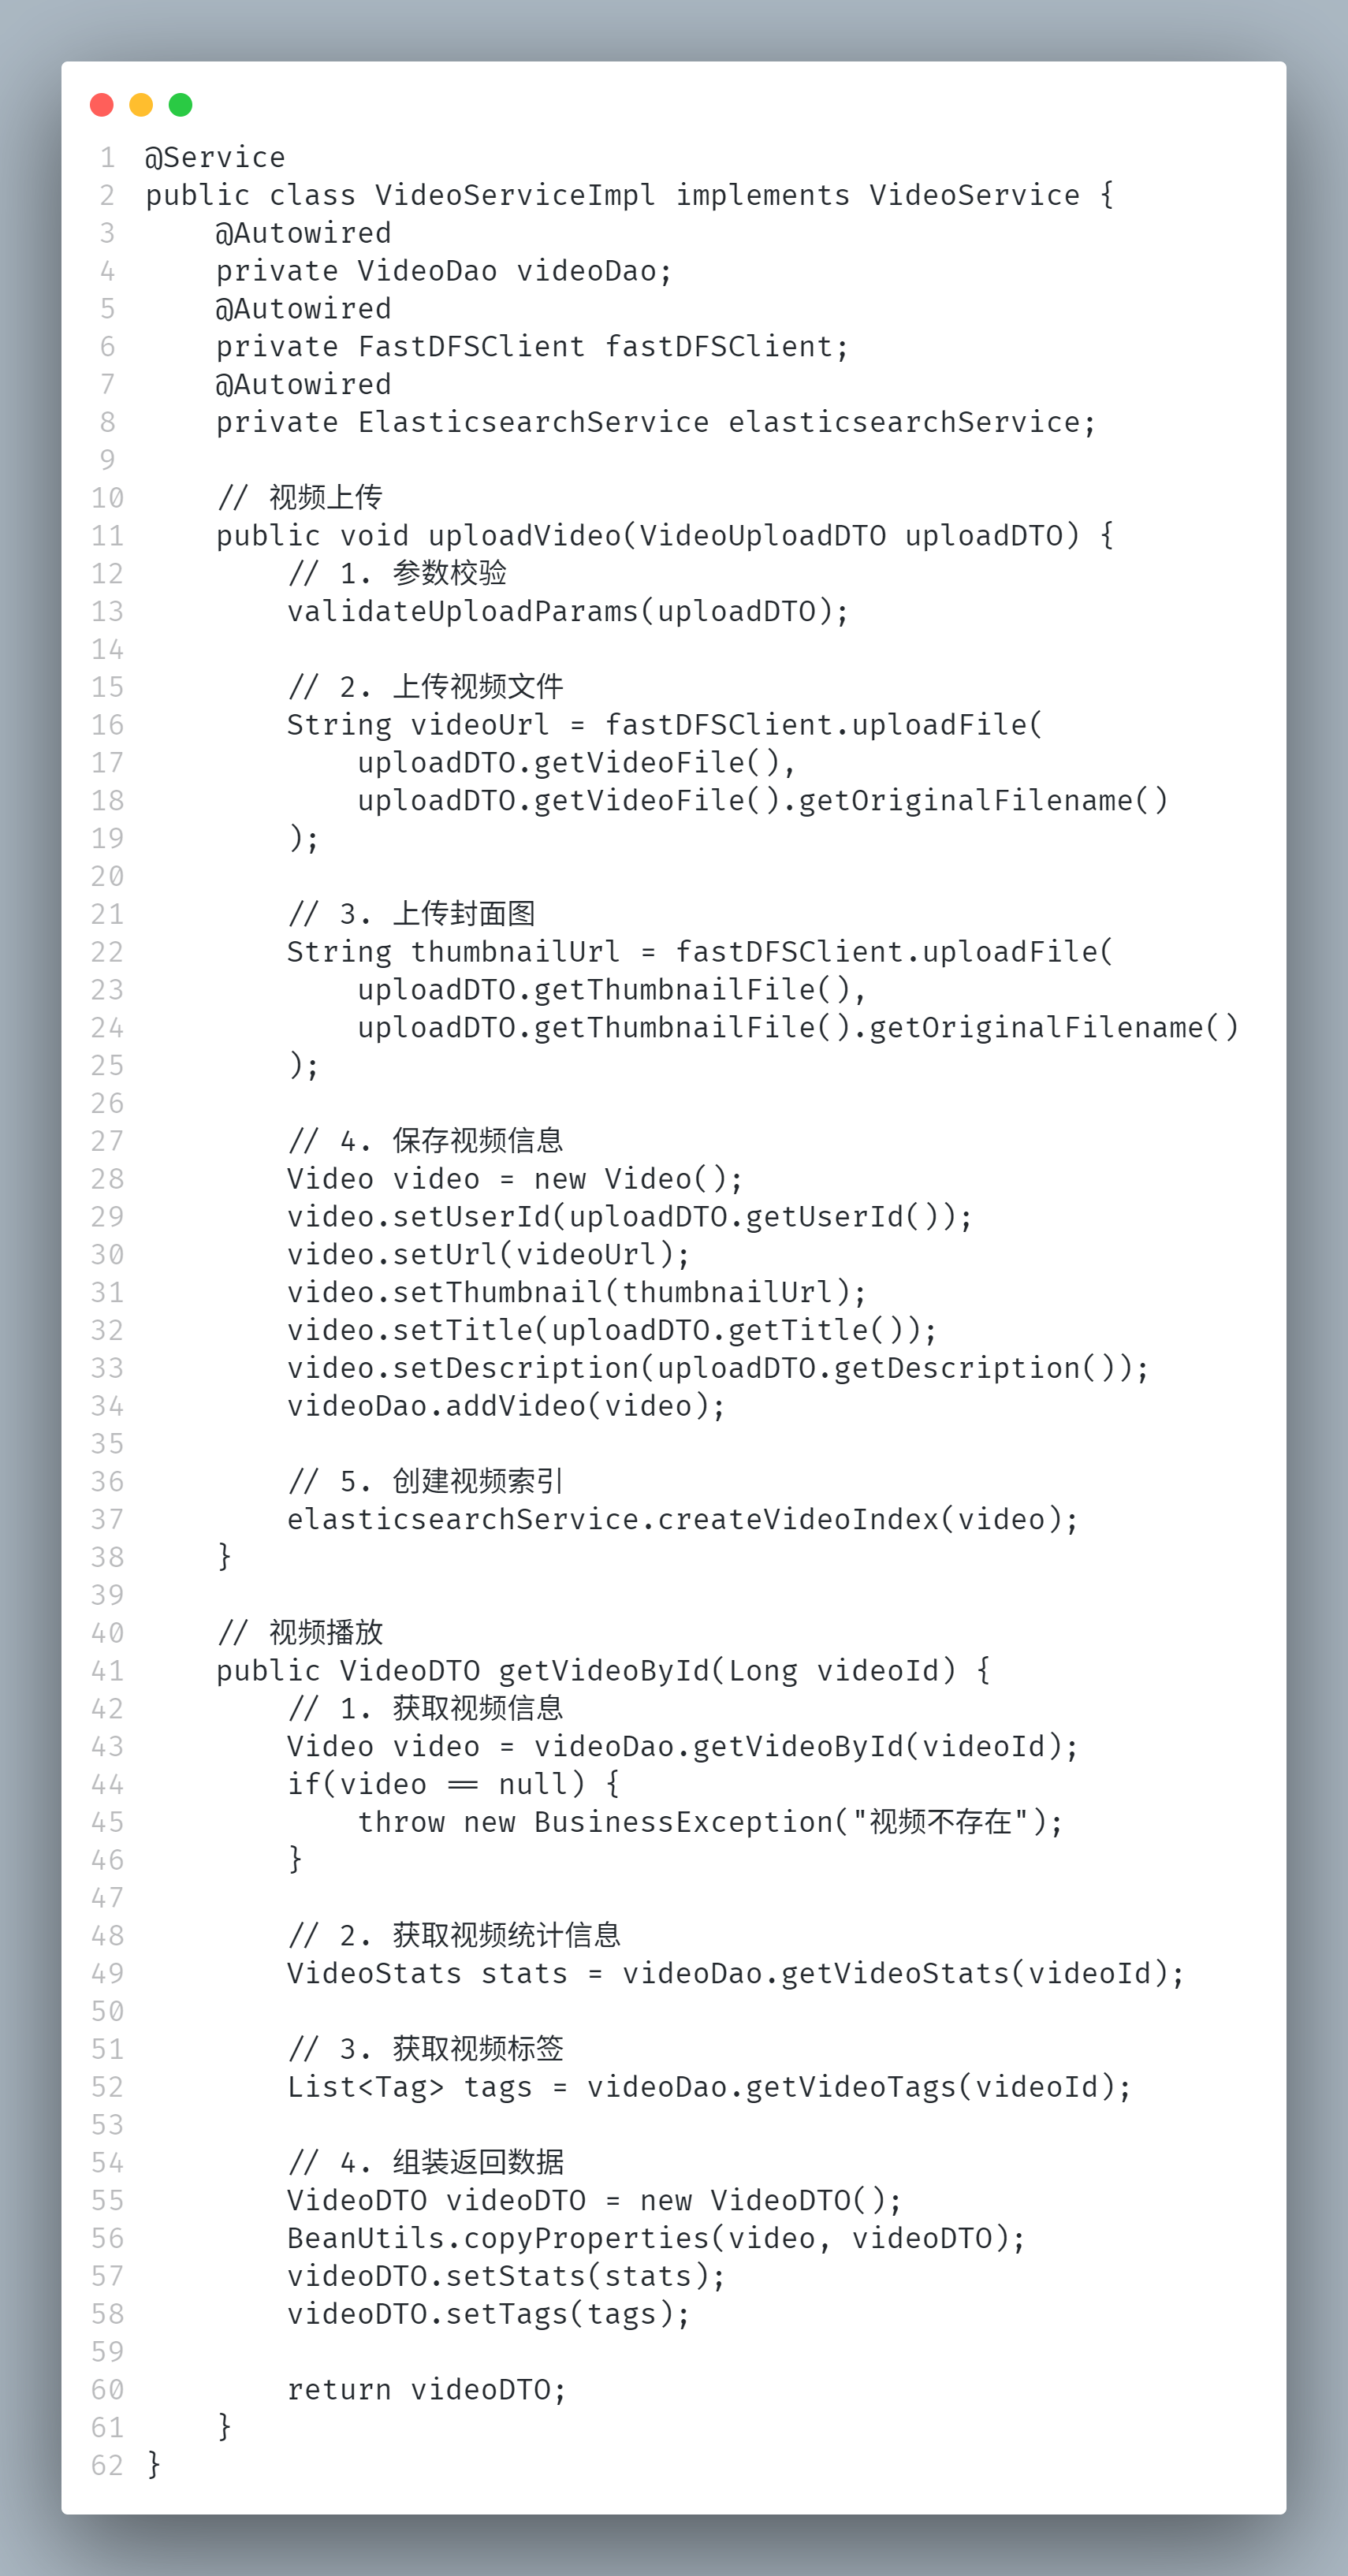
\includegraphics[width=0.75\textwidth]{视频模块.png}
    \caption{视频模块伪代码}
    \label{视频模块伪代码}
\end{figure}

视频上传功能,当用户发起视频上传请求时,系统会调用uploadVideo方法,具体的处理流程如下:
\begin{enumerate}[label=(\arabic*)]
    \item 参数校验:对用户提交的视频上传信息进行初步的合法性检查,确保上传的文件和相关参数完整且准确。
    \item 借助FastDFSClient将用户上传的视频文件存储到分布式文件系统中,并获取视频文件的存储路径。
    \item 封面图上传:同样使用FastDFSClient上传视频的封面图,并获取封面图的存储路径。
    \item 视频信息保存:创建一个Video 对象,将用户ID、视频路径、封面图路径、视频标题和描述等信息存储其中,然后通过VideoDao将视频信息持久化到数据库。
    \item 视频索引创建:调用ElasticsearchService在Elasticsearch中为该视频创建索引,以便后续的搜索和查询操作。
\end{enumerate}

视频播放功能,当用户请求播放视频时,系统会调用 getVideoById 方法,具体处理步骤如下:
\begin{enumerate}[label=(\arabic*)]
    \item 视频信息获取:通过 VideoDao 根据视频 ID 从数据库中获取对应的视频信息。若未找到该视频,则抛出 BusinessException 异常,提示 “视频不存在”。
    \item 视频统计信息获取:使用 VideoDao 获取该视频的统计信息,如播放量、点赞数等。
    \item 视频标签获取:通过 VideoDao 获取该视频的相关标签信息。
    \item 返回数据组装:创建一个 VideoDTO 对象,将视频信息、统计信息和标签信息进行整合,然后返回给用户,以便用户能够完整地获取视频相关信息进行播放。
\end{enumerate}

通过上述功能的实现,该视频服务模块为系统提供了完善的视频上传和播放服务,确保了视频数据的有效存储和展示。

\subsubsection{弹幕模块}
在弹幕服务模块中图\ref{弹幕模块伪代码},DanmuServiceImpl类是核心实现,它通过@Service注解被 Spring 容器识别为服务组件,实现了DanmuService接口,为弹幕的发送和获取功能提供了具体业务逻辑。
\begin{figure}[hbt]
    \centering
    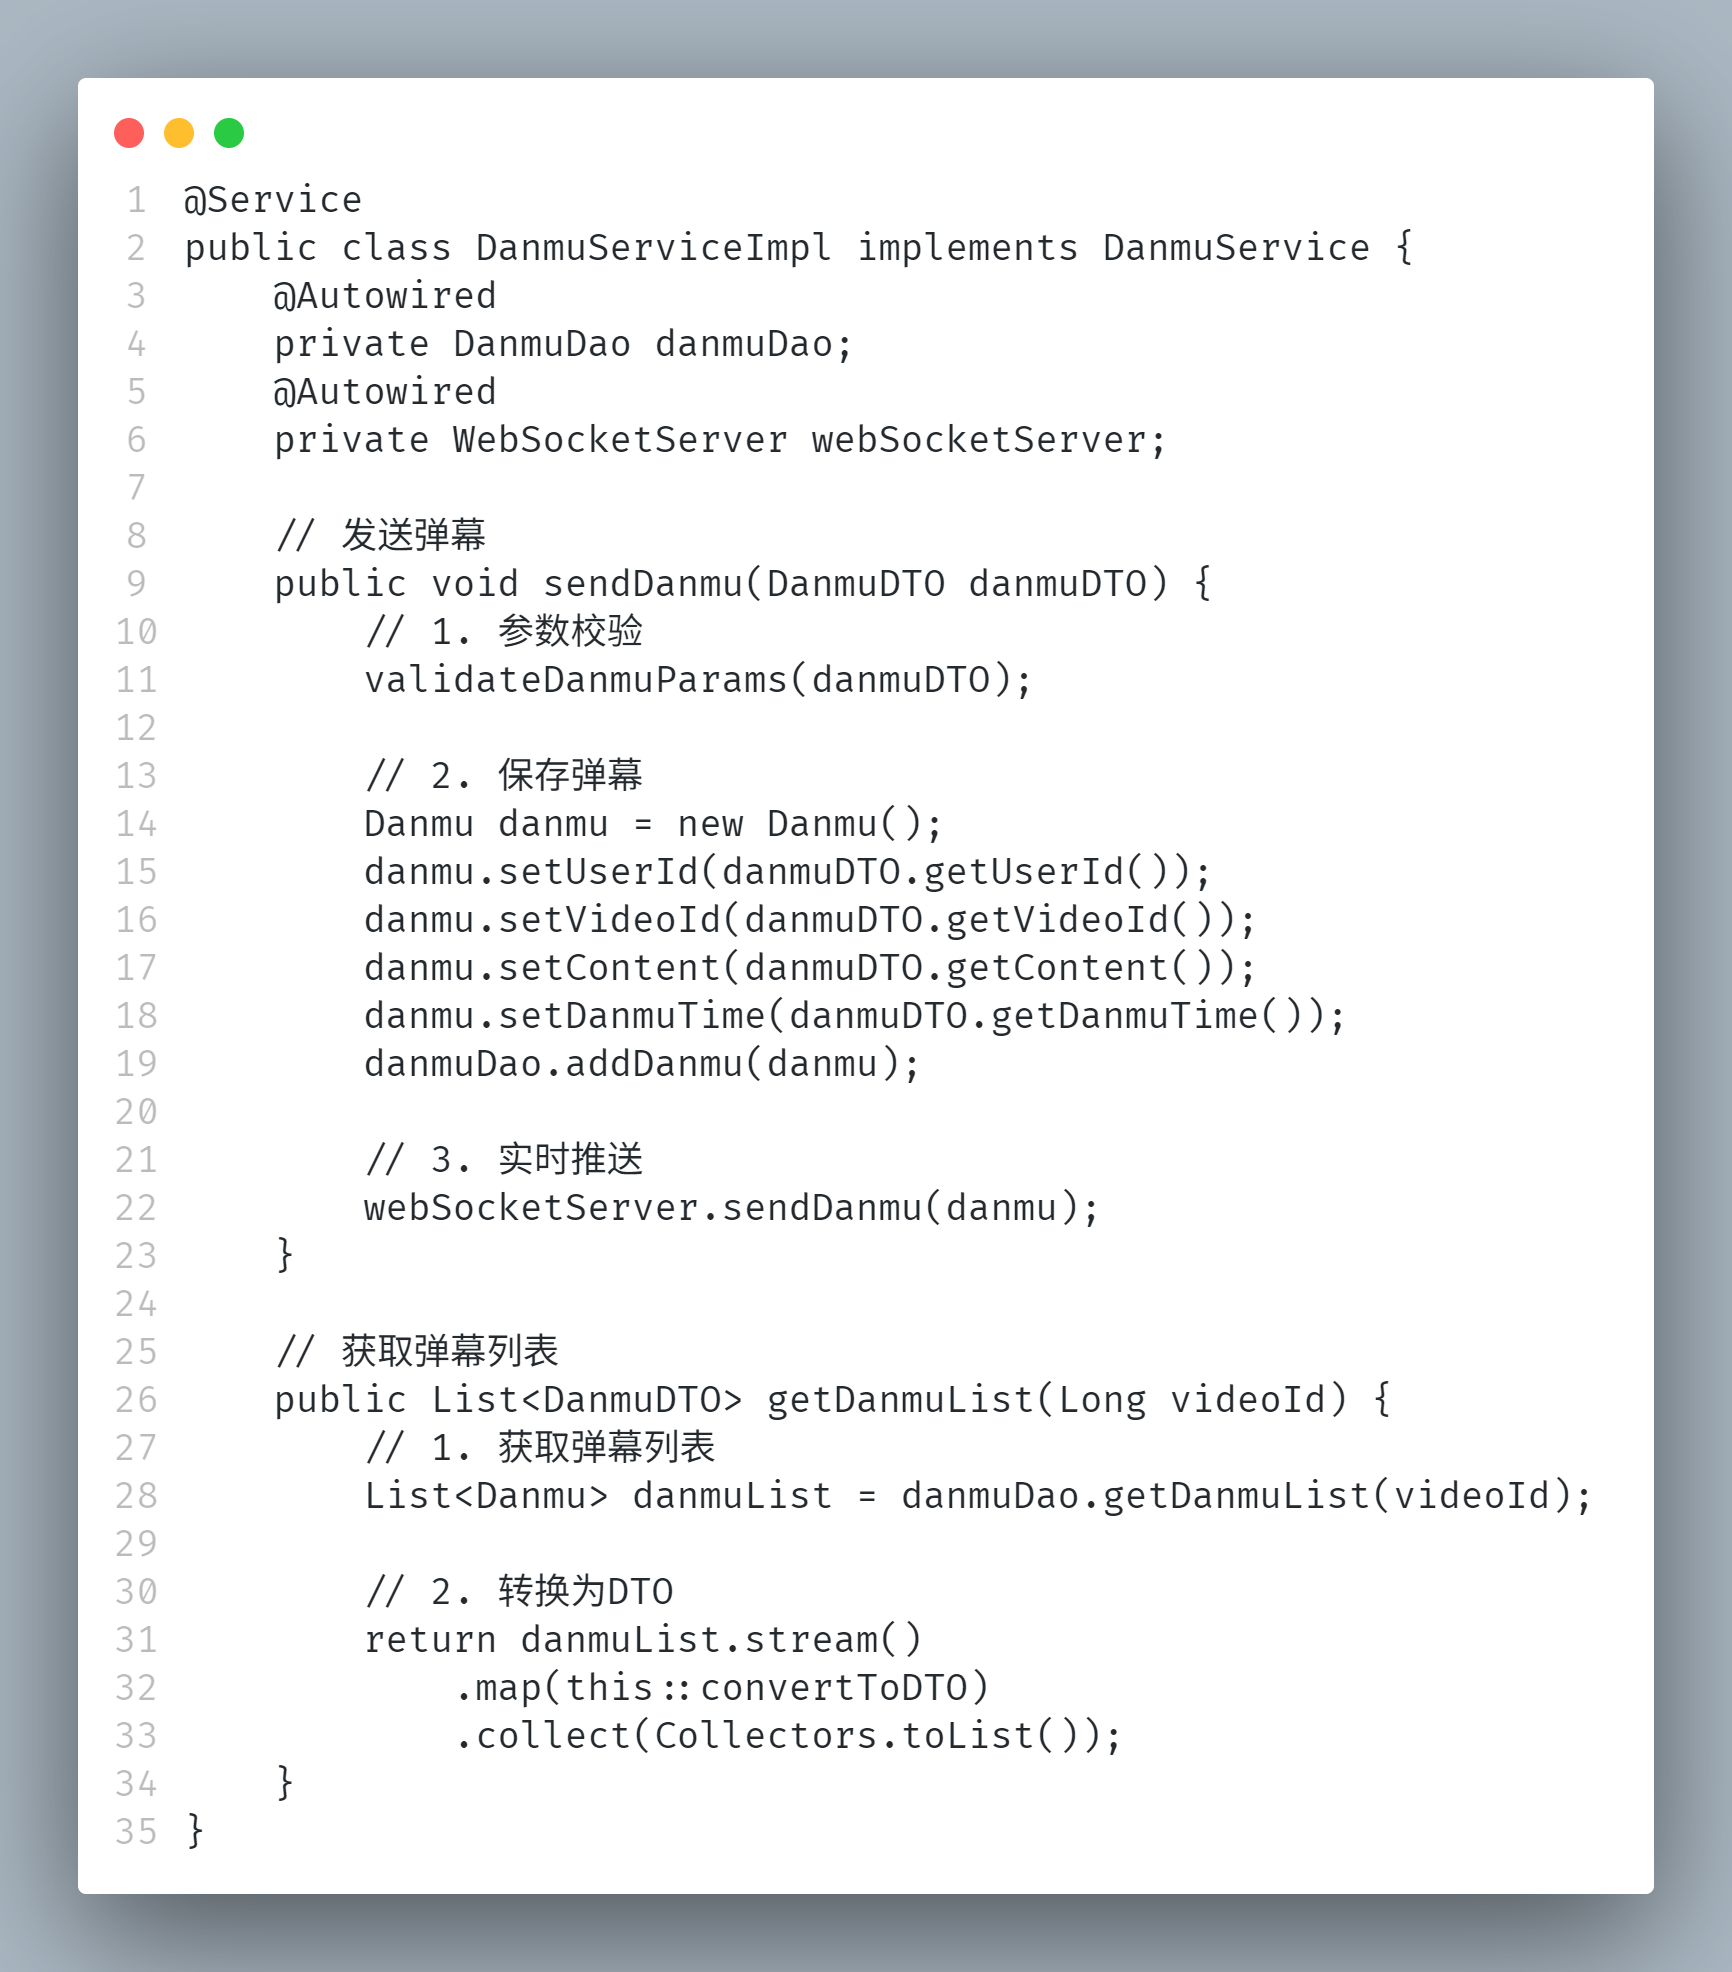
\includegraphics[width=0.75\textwidth]{弹幕模块.png}
    \caption{弹幕模块伪代码}
    \label{弹幕模块伪代码}
\end{figure}

弹幕发送功能,当用户发送弹幕时,系统会调用sendDanmu方法,详细处理步骤如下:
\begin{enumerate}[label=(\arabic*)]
    \item 参数校验:对用户发送的弹幕数据进行初步检查,确保数据的完整性和合法性,避免无效数据进入后续处理流程。
    \item 弹幕保存:创建一个Danmu对象,将用户ID、视频ID、弹幕内容以及弹幕发送时间等信息存入其中。接着,通过DanmuDao将该弹幕信息持久化到数据库,以便后续查询和分析。
    \item 实时推送:利用WebSocketServer将新发送的弹幕实时推送给正在观看该视频的其他用户,保证弹幕的即时性和交互性。
\end{enumerate}

弹幕列表获取功能,当需要获取某个视频的弹幕列表时,系统会调用getDanmuList方法,具体处理如下:
\begin{enumerate}[label=(\arabic*)]
    \item 弹幕数据查询:通过 DanmuDao 根据视频 ID 从数据库中查询该视频对应的所有弹幕信息。
    \item 数据转换:将查询到的Danmu对象列表转换为DanmuDTO列表。通过Java 8的Stream API对每个Danmu对象进行映射转换,最终收集为一个新的DanmuDTO列表并返回,以满足前端展示需求。
\end{enumerate}

通过上述功能实现,该弹幕服务模块为视频系统提供了高效的弹幕交互能力,保证了弹幕的存储、推送和展示功能的稳定运行。
\subsubsection{搜索模块}

如图\ref{搜索模块伪代码}在搜索服务模块中,SearchServiceImpl类起着关键作用,它通过 @Service注解被Spring容器识别为服务组件,实现了SearchService接口,为视频搜索和视频索引创建功能提供了具体的业务逻辑实现。
\begin{figure}[hbt]
    \centering
    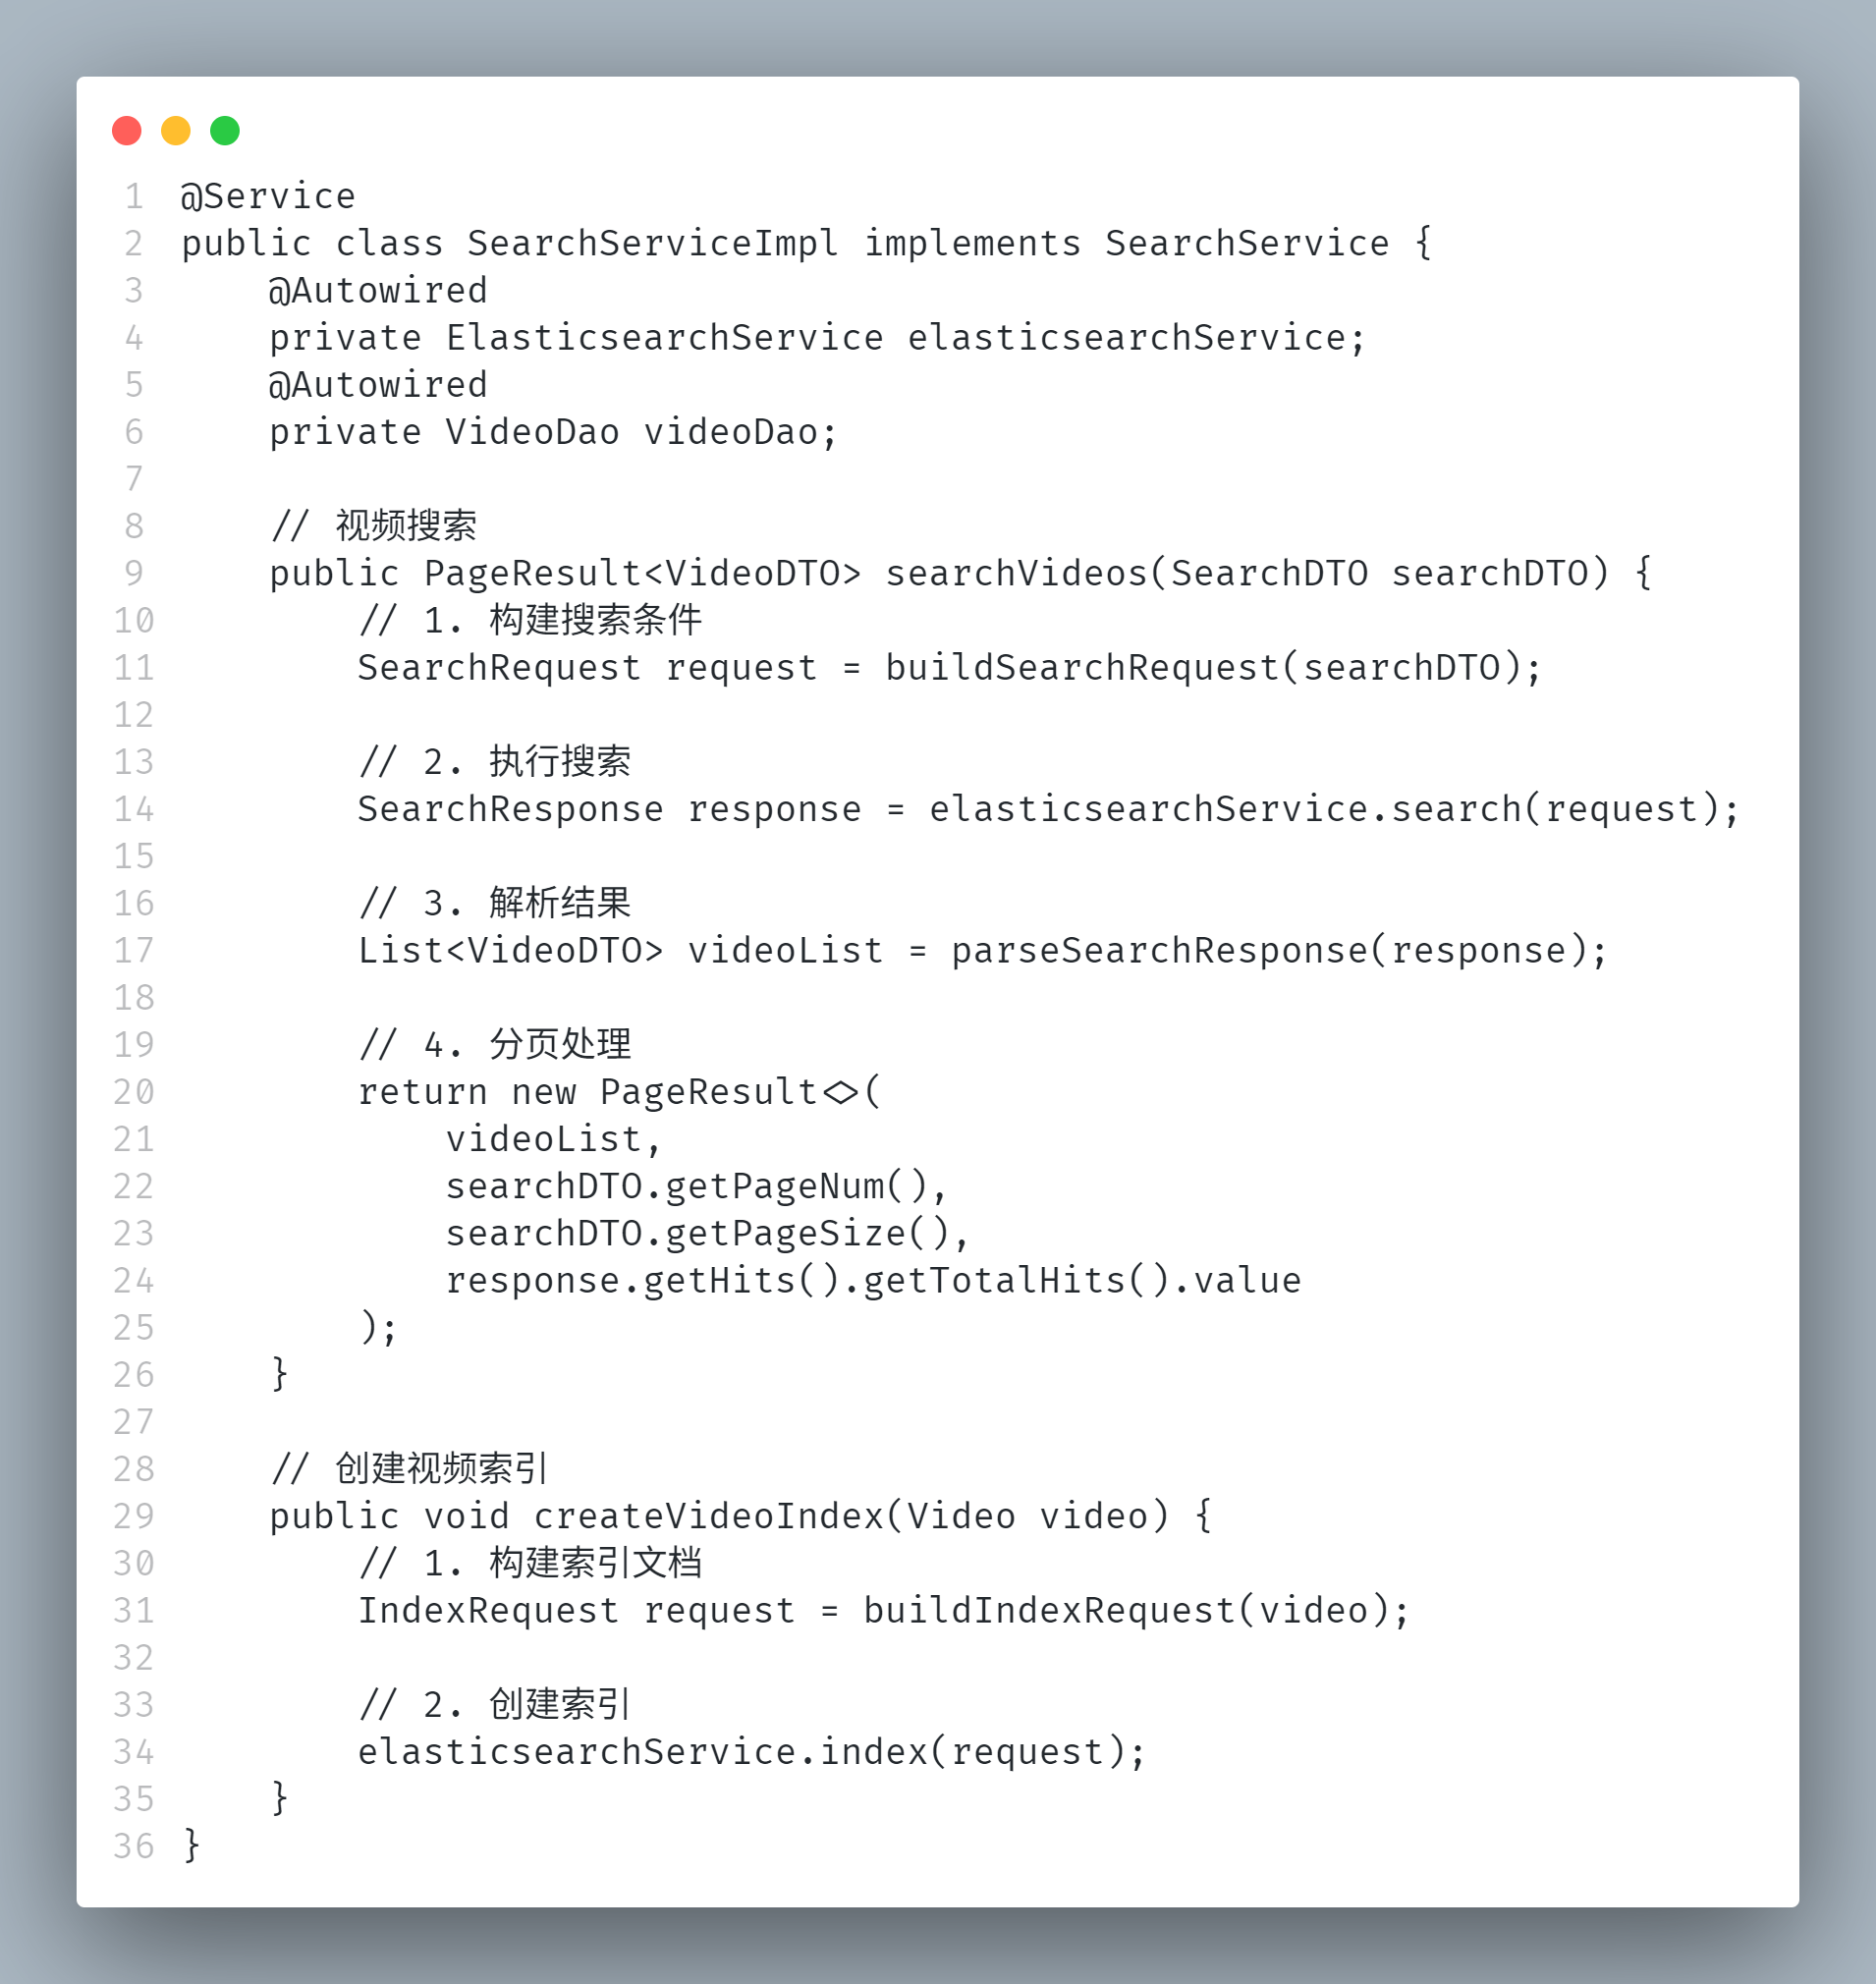
\includegraphics[width=0.75\textwidth]{搜索模块.png}
    \caption{搜索模块伪代码}
    \label{搜索模块伪代码}
\end{figure}

视频搜索功能,当用户发起视频搜索请求时,系统会调用searchVideos方法,具体处理流程如下:
\begin{enumerate}[label=(\arabic*)]
    \item 搜索条件构建:根据用户传入的SearchDTO对象,调用buildSearchRequest方法构建符合 Elasticsearch要求的搜索请求对象,该对象包含了用户的搜索条件。
    \item 执行搜索操作:将构建好的搜索请求对象传递给ElasticsearchService的search方法,在Elasticsearch中执行搜索操作,并获取搜索响应结果。
    \item 搜索结果解析:对Elasticsearch返回的搜索响应结果进行解析,调用parseSearchResponse方法将搜索结果转换为VideoDTO列表,方便后续处理和展示。
    \item 分页处理:将解析后的视频列表、用户请求的页码、每页数量以及搜索结果的总数量封装到PageResult对象中,实现搜索结果的分页展示,提高用户体验。
\end{enumerate}

视频索引创建功能,当需要为新视频创建索引时,系统会调用createVideoIndex方法,具体步骤如下:
\begin{enumerate}[label=(\arabic*)]
    \item 索引文档构建:根据传入的 Video 对象,调用 buildIndexRequest 方法构建 Elasticsearch 的索引请求对象,该对象包含了视频的相关信息。
    \item 索引创建操作:将构建好的索引请求对象传递给ElasticsearchService的index方法,在Elasticsearch中为该视频创建索引,以便后续能够对该视频进行搜索。
\end{enumerate}

通过上述功能的实现,该搜索服务模块为系统提供了高效的视频搜索和索引管理能力,确保用户能够快速准确地找到所需视频。

\newpage

\section{总结}

本研究聚焦于弹幕视频网站后端系统的设计与实现。随着网络技术进步,视频媒介蓬勃发展,用户对视频平台互动性提出更高要求,在此背景下确定研究方向。通过深入分析国内外视频平台发展现状,明确系统主要研究内容为打造集视频播放与弹幕交互等多功能于一体的后端系统。

在技术选型上,选用SpringBoot简化Java应用开发配置,MySQL进行数据存储管理,FastDFS实现分布式文件存储,WebSocket实现实时通信,Elasticsearch 提供搜索功能。经全面的需求分析,梳理出用户管理、视频管理、社交功能、权限管理、搜索功能和实时通信功能等功能性需求,以及性能、可用性、安全性、可拓展性和可维护性等非功能性需求。

系统设计环节,采用SpringBoot与SpringCloud构建微服务架构,进行系统分层设计和功能模块划分,并完成数据库概念结构和逻辑结构设计。系统实现过程中,详细介绍技术栈、开发环境与开发工具,成功搭建核心架构,完成用户、视频、弹幕、搜索等关键模块的开发。

经测试验证,该系统稳定可靠,能有效满足用户多样化需求,提升用户体验,为弹幕视频网站后端系统的发展提供了有效的技术方案和实践参考,也为后续研究和系统优化奠定了坚实基础。

\newpage


    \end{spacing}
}

%%%%%%%%%%%%%%%%%%%%%%%%%%%%%%%%%%%%%%%%%%%%%%%%%%
% 临时标签,用于编译时追踪正文末尾
%%%%%%%%%%%%%%%%%%%%%%%%%%%%%%%%%%%%%%%%%%%%%%%%%%

%%%%%%%%%%%%%%%%%%%%%%%%%%%%%%%%%%%%%%%%%%%%%%%%%%
% 后续内容
% --------------------------------------------%

% https://www.zhihu.com/question/29413517/answer/44358389 %
% 说明如下:
% secnumdepth 这个计数器是 LaTeX 标准文档类用来控制章节编号深度的。在 article 中,这个计数器的值默认是 3,对应的章节命令是 \subsubsection。也就是说,默认情况下,article 将会对 \subsubsection 及其之上的所有章节标题进行编号,也就是 \part, \section, \subsection, \subsubsection。LaTeX 标准文档类中,最大的标题是 \part。它在 book 和 report 类中的层级是「-1」,在 article 类中的层级是「0」。这里,我们在调用 \appendix 的时候将计数器设置为 -2,因此所有的章节命令都不会编号了。不过,一般还是会保留 \part 的编号的。所以在实际使用中,将它设置为 0 就可以了。

% 在修改过程中请注意不要破环命令的完整性

\renewcommand\appendix{\setcounter{secnumdepth}{-2}}
\appendix

% 主文件有代码去掉页眉章节编号的“.”,但这会因为bug导致无编号章节显示一个错误编号,所以这里在无编号章节之前再次重定义sectionmark。
\renewcommand{\sectionmark}[1]{\markright{#1}}

\setreference

%!TEX root = ../sztuthesis_main.tex

% 致谢
\begin{thankscontent}

\end{thankscontent}
 


\end{document}
